%================================================================
% H1 paper
%================================================================
\RequirePackage{lineno}
\documentclass[12pt]{article}


\usepackage{epsfig}
\usepackage{hhline}
\usepackage{amsmath}
\usepackage{amssymb}
\usepackage{color}
\usepackage{xspace}
%\usepackage{xfrac}
\usepackage{paralist} % compactitem
\usepackage{caption}
%\captionsetup[figure]{font=footnotesize,labelfont=footnotesize}
\captionsetup{font=small,labelfont=small}

\usepackage{bm} % 'bold' math symbols (better use \usepackage{newtxtext,newtxmath}, if available on latex distribution)
\usepackage{acronym}

%%%%%%%%%%%%% Comment the next two lines to remove the line numbering
\usepackage[]{lineno}
\linenumbers
%%%%%%%%%%%%%%

\usepackage{hyperref} % has to be last package loaded
\hypersetup{colorlinks=true, urlcolor=blue}
\usepackage{cite} % DB: enable also clickable references (must be loaded after hyperref)
\hypersetup{
%  colorlinks,
%  citecolor=blue,
%  linkcolor=red,
%  urlcolor=blue
  citecolor=[rgb]{0.,0.,0.5},
  linkcolor=[rgb]{0.6,0.,0.0},
  urlcolor=[rgb]{0.,0.,0.5}
  }


%%%%%%%%%%%%%% H1 preliminary
%\renewcommand{\topfraction}{1.0}
%\renewcommand{\bottomfraction}{1.0}
%\renewcommand{\textfraction}{0.0}
%\renewcommand{\arraystretch}{1.3} % make lines a bit larger for tables 
%%%%%%%%%%%%%%

%%%%%%%%%%%%%% H1 paper layout %%%%%%%%%%%%%%
\renewcommand{\topfraction}{1.0}
\renewcommand{\bottomfraction}{1.0}
\renewcommand{\textfraction}{0.0}
\renewcommand{\arraystretch}{1.25} % make lines a bit larger for tables
%\newlength{\dinwidth}
%\newlength{\dinmargin}
%\setlength{\dinwidth}{21.0cm}
%\textheight23.5cm \textwidth16.0cm
%\setlength{\dinmargin}{\dinwidth}
%\setlength{\unitlength}{1mm}
%\addtolength{\dinmargin}{-\textwidth}
%\setlength{\dinmargin}{0.5\dinmargin}
%\oddsidemargin -1.0in
%\addtolength{\oddsidemargin}{\dinmargin}
%\setlength{\evensidemargin}{\oddsidemargin}
%\setlength{\marginparwidth}{0.9\dinmargin}
\marginparsep 8pt \marginparpush 5pt
\topmargin -42pt
\headheight 12pt
\headsep 30pt \footskip 24pt
\parskip 3mm plus 2mm minus 2mm

% do not indent first line of paragraph!
%\setlength{\parindent}{0pt}
\usepackage{parskip}
%%%%%%%%%%%%%%%%%%%%%%%%%%%%%%%%%%%%%%%%%%%%%




%%% contains utf-8, see: http://inspirehep.net/info/faq/general#utf8
%%% add \usepackage[utf8]{inputenc} to your latex preamble
\usepackage[utf8]{inputenc}
%\bibliographystyle{plain}%Choose a bibliograhpic style          
\bibliographystyle{utphys}%Choose a bibliograhpic style          

\newlength{\dinwidth}
\newlength{\dinmargin}
\setlength{\dinwidth}{21.0cm}
\textheight23.5cm \textwidth16.0cm
\setlength{\dinmargin}{\dinwidth}
\setlength{\unitlength}{1mm}
\addtolength{\dinmargin}{-\textwidth}
\setlength{\dinmargin}{0.5\dinmargin}
\oddsidemargin -1.0in
\addtolength{\oddsidemargin}{\dinmargin}
\setlength{\evensidemargin}{\oddsidemargin}
\setlength{\marginparwidth}{0.9\dinmargin}
\marginparsep 8pt \marginparpush 5pt
\topmargin -42pt
\headheight 12pt
\headsep 30pt \footskip 24pt
\parskip 3mm plus 2mm minus 2mm
\setlength{\parindent}{0.0cm} 
\newcommand{\picob}{\mbox{{\rm ~pb}}}
\newcommand{\QQ}  {\mbox{${Q^2}$}}

\newcommand{\NNLOJET}{NNLO\protect\scalebox{0.8}{JET}\xspace}

%===============================title page=============================

% Some useful tex commands
%
%\def\GeV{\hbox{$\;\hbox{\rm GeV}$}}
%\def\MeV{\hbox{$\;\hbox{\rm MeV}$}}
%\def\TeV{\hbox{$\;\hbox{\rm TeV}$}}

\newcommand{\pb}{\rm pb}
\newcommand{\cm}{\rm cm}
\newcommand{\hdick}{\noalign{\hrule height1.4pt}}

\begin{document}
\pagestyle{empty}

\newcommand{\GeVsq}{\ensuremath{\mathrm{GeV}^2} }
\newcommand{\GeV}{\ensuremath{\mathrm{GeV}} }
\newcommand{\pt}{\ensuremath{P_{T}}}
\newcommand{\PP}{\ensuremath{\mathcal{P}}}
%\newcommand{\ptAvg}{\ensuremath{\langle P_T^{jet}\rangle}}
\newcommand{\ptjone}{\ensuremath{p_{\mathrm{T}}^{\ast,\rm jet1}}\xspace}
\newcommand{\ptjtwo}{\ensuremath{p_{\mathrm{T}}^{\ast,\rm jet2}}\xspace}
\newcommand{\Qsq}{\ensuremath{Q^{2}}}
%% unfolding
\newcommand{\chisq}{\ensuremath{\chi^{2}}}
\newcommand{\chisqA}{\ensuremath{\chi_{\rm A}^{2}}}
\newcommand{\chisqL}{\ensuremath{\chi_{\rm L}^{2}}}
\newcommand{\ndf}{\ensuremath{n_{\rm dof}}}
\newcommand{\A}{\ensuremath{\bm{A}}}
\newcommand{\V}{\ensuremath{\bm{V}}}
\newcommand{\B}{\ensuremath{\bm{B}}}
\newcommand{\J}{\ensuremath{\bm{J}}}
\newcommand{\N}{\ensuremath{\bm{N}}}
\newcommand{\LL}{\ensuremath{\bm{L}}}

\newcommand{\etajet}{\ensuremath{\eta_{\rm lab}^{\rm jet}}}
\newcommand{\ptjet}{\ensuremath{P_{\rm T}^{\rm jet}}}
\newcommand{\meanpt}{\ensuremath{\langle P_{\rm T} \rangle}}
\newcommand{\etalab}{\ensuremath{\eta_{\rm lab}^{\rm jet}}}
\newcommand{\Mjj}{\ensuremath{m_{12}}}
\newcommand{\meanptdi}{\ensuremath{\langle P_{\mathrm{T}} \rangle_{2}}\xspace}
\newcommand{\meanpttri}{\ensuremath{\langle P_{\mathrm{T}} \rangle_{3}}\xspace}
\newcommand{\mz}{\ensuremath{m_{\rm Z}}\xspace}
\newcommand{\as}{\ensuremath{\alpha_{\rm s}}\xspace}
\newcommand{\asmz}{\ensuremath{\as(\mz)}\xspace}
\newcommand{\asmzPDF}{\ensuremath{\as^{\rm PDF}(\mz)}\xspace}
\newcommand{\asmzf}{\ensuremath{\as^{\Gamma}(\mz)}\xspace}
\newcommand{\tilmu}{\ensuremath{\tilde{\mu}}\xspace}
\newcommand{\etal}{{\it{et al.}}}
\newcommand{\mur}{\ensuremath{\mu_{\rm R}}\xspace}
\newcommand{\muf}{\ensuremath{\mu_{\rm F}}\xspace}
\newcommand{\mup}{\ensuremath{\mu_{0}}\xspace}
\newcommand{\murf}{\ensuremath{\mu_{\rm R/F}}\xspace}
\newcommand{\asmur}{\ensuremath{\alpha_{\rm s}(\mur)}\xspace}
\newcommand{\chad}{\ensuremath{c_{\rm had}}\xspace}
\newcommand{\ord}{\ensuremath{\mathcal{O}}\xspace}

\renewcommand{\contentsname}{Content \footnotesize (only for editorial purposes)}
\newcommand{\invpb}{\ensuremath{{\rm pb}^{-1}}\xspace}

\newcommand{\pom}{\ensuremath{I\!\!P}}
\newcommand{\reg}{\ensuremath{I\!\!R}}
\newcommand{\mxq}{\ensuremath{M_{\rm X}^{2}}\xspace}
\newcommand{\mx}{\ensuremath{M_{\rm X}}\xspace}
\newcommand{\MY}{\ensuremath{M_{\rm Y}}\xspace}
\newcommand{\xpom}{\ensuremath{x_{\pom}}\xspace}
\newcommand{\zpom}{\ensuremath{z^{\rm obs}_{\pom}}\xspace}
\newcommand{\zint}{\ensuremath{z_{\pom}}\xspace}
\newcommand{\xbj}{\ensuremath{x_{\mathrm{Bj}}\xspace}}

% The DPDFs
\newcommand{\DPDF}{H1 Fit2019 NNLO (prel.)\xspace}
\newcommand{\DPDFFitA}    {H1FitA\xspace}
\newcommand{\DPDFFitB}    {H1FitB\xspace}
\newcommand{\DPDFFitJets} {H1FitJets\xspace}
\newcommand{\DPDFZSJ} {ZEUSSJ\xspace}
\newcommand{\DPDFMRW} {MRW\xspace}

% The data
\newcommand{\HIcomb} {H1comb-LRG\xspace}
\newcommand{\HILowEa} {H1-LowE-225\xspace}
\newcommand{\HILowEb} {H1-LowE-252\xspace}
% the jet data
\newcommand{\HERAI} {\protect\scalebox{0.8}{(HERA~{1})}}
\newcommand{\HERAII} {\protect\scalebox{0.8}{(HERA~{2})}}
\newcommand{\LowEP} {\protect\scalebox{0.8}{($300\,\GeV$)}}
\newcommand{\HLRG}  {H1 LRG \HERAII\xspace}
\newcommand{\HVFPS} {H1 VFPS \HERAII\xspace}
\newcommand{\HFPS}  {H1 FPS \HERAII\xspace}
\newcommand{\HLRGI} {H1 LRG \HERAI\xspace}
\newcommand{\ZLRG}  {ZEUS LRG \HERAI\xspace}
\newcommand{\HLRGEp}{H1 LRG \LowEP\xspace}


% % % Journal macro
% % \def\Journal#1#2#3#4{{#1}~{\bf #2} (#3) #4}
% % %\def\NCA{\em Nuovo Cimento}
% % %\def\NIM{\em Nucl. Instrum. Methods}
% % %\def\NIMA{{\em Nucl. Instrum. Methods} {\bf A}}
% % %\def\NPB{{\em Nucl. Phys.}   {\bf B}}
% % %\def\PLB{{\em Phys. Lett.}   {\bf B}}
% % %\def\PRL{\em Phys. Rev. Lett.}
% % %\def\PRD{{\em Phys. Rev.}    {\bf D}}
% % %\def\ZPC{{\em Z. Phys.}      {\bf C}}
% % %\def\EJC{{\em Eur. Phys. J.} {\bf C}}
% % %\def\CPC{\em Comp. Phys. Commun.}
% % %
% % \def\NPB{Nucl. Phys.~}
% % \def\PRL{Phys. Rev. Lett.~}
% % \def\EPJC{Eur. Phys. J.~}
% % \def\PLB{Phys. Lett.~}
% % \def\NIM{Nucl. Instrum. Meth.~}
% % \def\PRD{Phys. Rev.~}
% % \def\JHEP{JHEP~}
% % \def\PROC{Conf. Proc.~}
% % \def\CPC{Comp. Phys. Commun.~}
% % 




%%%%%%%%%%%%%%%%%%%%%%%%%%%%%%%%%%%%%%% title page %%%%%%%%%%%%%%%%%%%%%%%%%%%%%%%%%%%%%%%%
\begin{titlepage}
\noindent
\begin{flushleft}
% {\tt H1prelim-19-013 DRAFT ! \hfill    ISSN abcd-abcd} \\
{\tt H1prelim-19-013} \\
{\tt April 2019}                  \\
\end{flushleft}

\noindent
%Date:   ~   \ \ April 2019 %31.\,08.\,2017      \\
%Version:~   0.0 \\
%Editors:~   D.~Britzger, R.~\v{Z}leb\v{c}\'{i}k (daniel.britzger@desy.de, zlebcr@mail.desy.de) \\
%Referees:  K.~Cerny, L.~Favart \\
%Final reading scheduled for ....         \\
\noindent

\vspace{1cm}
\begin{center}
\begin{Large}

{\bf
  A determination of diffractive parton distribution functions from
  H1 inclusive diffractive deep-inelastic scattering data and H1 diffractive dijet cross section data
  in next-to-next-to-leading order QCD
}

\vspace{1.5cm}

H1 Collaboration%\footnote{}

\end{Large}
\end{center}

\vspace{1.5cm}


\begin{abstract}
\noindent
%Abstract
A new combined fit of diffractive parton distribution functions (DPDFs) to the H1 inclusive neutral-current and dijet production data in diffractive deep-inelastic scattering (DDIS) at next-to-next-to-leading order accuracy (NNLO) is presented.
Compared to the previous HERA fits, the presented study includes the high-precision H1 HERA-II data, which represents 40~times higher luminosity for inclusive DDIS data sample and 6~times higher luminosity for the jet data, than previous studies by H1.
In addition to the inclusive DDIS data at the nominal centre-of-mass energy $\sqrt{s}=319$, also the inclusive data at 252 and 225\,GeV are included into the fit.
The inclusion of the most comprehensive dijet cross section data, together with their NNLO predictions, provide enhanced constraints to the gluon component of the DPDF.
The extracted DPDFs are compared to the alternative existing DPDFs at NLO accuracy, and are used to predict cross sections for a large number of the available dijet measurements.
\noindent
\end{abstract}


\begin{center} Submitted to DIS19 conference, Torino \end{center}

\end{titlepage}
%% ------------------------------------------------------------------------------ %%





%% ------------------------------------------------------------------------------ %%
\clearpage
%\tableofcontents
%\clearpage
%% ------------------------------------------------------------------------------ %%

\pagestyle{plain} %% page numbers


%%%%%%%%%%%%%%%%%%%%%%%%%%%%%%%%%%%%%%%%%%%%%%%%%%%%%%%%%%%%
%                    Introduction
%%%%%%%%%%%%%%%%%%%%%%%%%%%%%%%%%%%%%%%%%%%%%%%%%%%%%%%%%%%%
\section{Status of document}
The present document is just a collection of plots, for the preliminary request on 28.3.2019.
Further text, and references still have to be included.

\section{Introduction}

%Diffractive processes in deep-inelastic scattering, $ep \to eXY$, where the final state systems $X$ and $Y$ are separated in rapidity, have been studied extensively at the electron-proton collider HERA [1].
%%
%The forward system $Y$ consists of the leading proton, which stays intact after the collisions, but may also contain its low mass dissociation.
%%
%Between the systems $X$ and $Y$ a depleted region without any hadronic activity is observed, the so-called large rapidity gap
%(LRG).
%%
%This is a consequence of the vacuum quantum numbers of the diffractive exchange which is often referred to as a pomeron (IP).
%%
%Experimentally, the diffractive events can be selected either by requiring a rapidity region in the direction of the proton beam without any hadronic activity (LRG method) or by direct detection of the leading proton using dedicated spectrometers.
%%
%In the second case, the system $Y$ is free of any diffractive dissociation.
%
%The deep-inelastic scattering is characterized by a virtuality $Q^2$ ($Q^2 >> \lambda_{QCD}$) which represents the hard scale of the process.
%The factorisation theorem for DDIS \cite{Collins:1997sr} [...].




%%%%%%%%%%%%%%%%%%%%%%%%%%%%%%%%%%%%%%%%%%%%%%%%%%%%%%%%%%%%
%                    Data
%%%%%%%%%%%%%%%%%%%%%%%%%%%%%%%%%%%%%%%%%%%%%%%%%%%%%%%%%%%%
%\clearpage
\section{Data selection}
For the present analysis measurements of jet cross sections and inclusive DDIS cross sections in lepton-proton collisions performed by the H1 experiment at HERA are exploited.
%
Compared to the previous H1 fits \cite{Aktas:2006hy,Aktas:2007bv} which where based on the HERA~I data from years 1996-1997, the new fit includes the HERA-II data for both the inclusive DIS and the jet production in DIS.
These data has about 40~times higher luminosity in case of inclusive production and 6~times higher for the dijets.
These data covers the region of $|t| < 1\,\text{GeV}^2$ of the proton four-momentum transfer and $M_Y < 1.6\,\text{GeV}$.
For the present study, data based on the large rapidity gap selection method are used, and
the selected inclusive neutral-current DDIS data samples are summarised in table~\ref{tab:datasetsDDIS}.

\begin{table}[tbhp]
  \footnotesize
  %\scriptsize
  \begin{center}
    \begin{tabular}{cccc}
%      \multicolumn{6}{c}{\bf Kinematic range of H1 jet data} \\
      \hline
      \multicolumn{1}{c}{Data set} & $\sqrt{s}$ & int. $\mathcal{L}$ & DIS kinematic  \\  
      \multicolumn{1}{c}{[ref.]}  & $[\GeV]$   & $[{\rm pb}^{-1}]$  &  range         \\   
      \hline
      \HIcomb      & 319 & 336.6 & $8.5<\Qsq<1600\,\GeVsq$   \\
      \HILowEa     & 252 & 5.2   & $8.5<\Qsq<44\,\GeVsq$   \\
      \HILowEb     & 225 & 8.5   & $8.5 <\Qsq<44\,\GeVsq $   \\
      \hline
    \end{tabular}
    \caption{
      Summary of inclusive NC DDIS data samples selected for the present DPDF fit.
      On the of the $Q^2 > 8.5\;\GeVsq$ cut the $M_X > 2\,\GeV$ is applied to avoid resonance region.
    }
    \label{tab:datasetsDDIS}
    \end{center}
\end{table}


The combined data set \HIcomb\ was obtained from a combination of six individual data sets as summarised in table~\ref{tab:datasetsComb}
\begin{table}[tbhp]
  \footnotesize
  %\scriptsize
  \begin{center}
    \begin{tabular}{cccc}
%      \multicolumn{6}{c}{\bf Kinematic range of H1 jet data} \\
      \hline
      \multicolumn{1}{c}{Data set} & $\sqrt{s}$ & int. $\mathcal{L}$ & DIS kinematic  \\  
      \multicolumn{1}{c}{[ref.]}  & $[\GeV]$   & $[{\rm pb}^{-1}]$  &  range         \\   
      \hline
      1999 MB   & 319 & 3.5  & $3<\Qsq<25\,\GeVsq$   \\
      1999-2000 & 319 & 34.3 & $10< \Qsq<105\,\GeVsq $   \\
      2004-2007 & 319 & 336.6 & $10< \Qsq<105\,\GeVsq $   \\
      \hline
      1997 MB   & 300 & 2.0 & $3<\Qsq<13.5\,\GeVsq$   \\
      1997 all  & 300 & 10.6 & $13.5<\Qsq<105\,\GeVsq$   \\
      1999-2000 & 319 & 61.6 & $133\,\GeVsq < \Qsq $   \\
      \hline
    \end{tabular}
    \caption{
      Summary of the individual data sets that went into the \HIcomb data set, which is then selected for the present DPDF fit.
    }
    \label{tab:datasetsComb}
    \end{center}
\end{table}

In addition to the inclusive NC DDIS data, also cross sections for dijet production in NC DDIS are considered for the present DPDF fit.
%
Albeit there is considerable variety of different measurements, for the present fit we select only only the HERA-II dijet cross section data based on LRG selection, due to its outstanding statistical uncertainty in comparison to other analysis, and since this analysis was performed double-differentially as a function of \Qsq\ and the average transverse momentum of the two leading jets, \meanpt.
The selected dijet cross section data is summarised in table~\ref{tab:datasetsJets}.


\begin{table*}[tbhp]
  \scriptsize
  \begin{center}
    \begin{tabular}{ccccc}
%      \multicolumn{5}{c}{\bf Summary of experimental data sets} \\                                                                                                                                                                    
            \hline
            {\bf Data Set}  & {\boldmath{$\mathcal{L}$}}
            & {\bf DIS} & {\bf Dijet} & {\bf Diffractive}   \\     %                                                                                                                                                                   
            & [{\invpb}]
            & {\bf range} & {\bf range} & {\bf range} \\
      \hline
%      \HFPS \cite{Aaron:2011mp} &  156.6 &  $4<\Qsq<110\,\GeVsq$ & $\ptjone>5\,\GeV$ & $\xpom<0.1$ \\
%            &(581ev)& $0.05 < y < 0.7$ & $\ptjtwo>4.0\,\GeV$& $|t|<1\,\GeVsq$ \\
%            & & & $-1<\etalab<2.5$& $\MY= m_P $ \\
%      \hline
%      \HVFPS \cite{Andreev:2015cwa} &  50 &  $4<\Qsq<80\,\GeVsq$ & $\ptjone>5.5\,\GeV$ & $0.010<\xpom<0.024$ \\
%            &(550ev)& $0.2 < y < 0.7$ & $\ptjtwo>4.0\,\GeV$& $|t|<0.6\,\GeVsq$ \\
%            & & & $-1<\etalab<2.5$ & $\MY= m_P $ \\
%      \hline
      \HLRG \cite{Andreev:2014yra} &  290 &  $4<\Qsq<100\,\GeVsq$ & $\ptjone>5.5\,\GeV$ & $\xpom<0.03$ \\
            &($\sim$15000ev)& $0.1 < y < 0.7$ & $\ptjtwo>4.0\,\GeV$& $|t|<1\,\GeVsq$ \\
            & & & $-1<\etalab<2$ & $\MY<1.6 \, \GeV$ \\
      \hline
%      \HLRGI \cite{Aktas:2007bv} & 51.5 &  $4<\Qsq<80\,\GeVsq$ & $\ptjone>5.5\,\GeV$ & $\xpom<0.03$ \\
%            &(2723ev)& $0.1 < y < 0.7$ & $\ptjtwo>4.0\,\GeV$& $|t|<1\,\GeVsq$ \\
%            & & & $-3<\eta^{*\mathrm{jet}}<0$ & $\MY<1.6 \, \GeV$ \\
%      \hline
%      \HLRGEp \cite{Aktas:2007hn} &  18 &  $4<\Qsq<80\,\GeVsq$ & $\ptjone>5\,\GeV$ & $\xpom<0.03$ \\
%             &(322ev)& $165 < W < 242\,\GeV$ & $\ptjtwo>4.0\,\GeV$& $|t|<1\,\GeVsq$ \\
%             & & $(0.30 < y < 0.65)$& $-1<\etalab<2$& $\MY<1.6 \, \GeV$ \\
%             & &  & $-3<\eta^{*\mathrm{jet}}<0$&  \\
%      \hline
%      \ZLRG \cite{Chekanov:2007aa} &  61 &  $5<\Qsq<100\,\GeVsq$ & $\ptjone>5\,\GeV$ & $\xpom<0.03$ \\
%            &(5539ev)& $100 < W < 250\,\GeV$ & $\ptjtwo>4.0\,\GeV$& $|t|<1\,\GeVsq$ \\
%            & &  $(0.10 < y < 0.62)$  & $-3.5<\eta^{*\mathrm{jet}}<0$ & $\MY = m_P$ \\
%      \hline
    \end{tabular}
    \caption{
      Summary of the dijet data sets used in the present DPDF analysis.
%      The first column represents the data set label and the second
%      shows the integrated luminosity and the number of events of the
%      given data set.
%      The other columns summarise the definition of the phase space of
%      the given data.
%      In cases, where the DIS phase space is defined in terms of $W$,
%      the corresponding range in $y=W^2/s$ is shown.
%      All measurements have in common a requirement of $n_{\rm jets}
%      \geq 2$, which is applied after identifying the two leading
      %      jets.
      From the \HLRG\ dijet measurement, the double-differential cross sections as functions of \Qsq\ and \meanpt\ are selected.
    }
    \label{tab:datasetsJets}
    \end{center}
\end{table*}



%%%%%%%%%%%%%%%%%%%%%%%%%%%%%%%%%%%%%%%%%%%%%%%%%%%%%%%%%%%%
%                    Theory
%%%%%%%%%%%%%%%%%%%%%%%%%%%%%%%%%%%%%%%%%%%%%%%%%%%%%%%%%%%%
%\clearpage
%\begin{boldmath}
%\section{Theory}
%\end{boldmath}
%\label{sec:theory}


%%%%%%%%%%%%%%%%%%%%%%%%%%%%%%%%%%%%%%%%%%%%%%%%%%%%%%%%%%%%
%                    Methodology
%%%%%%%%%%%%%%%%%%%%%%%%%%%%%%%%%%%%%%%%%%%%%%%%%%%%%%%%%%%%
%\section{Methodology}
%\label{sec:method}


%%%%%%%%%%%%%%%%%%%%%%%%%%%%%%%%%%%%%%%%%%%%%%%%%%%%%%%%%%%%
%                      Results
%%%%%%%%%%%%%%%%%%%%%%%%%%%%%%%%%%%%%%%%%%%%%%%%%%%%%%%%%%%%
\section{Results}
\label{sec:results}


\begin{table}[tbhp]
  \footnotesize
  %\scriptsize
  \begin{center}
    \begin{tabular}{lcc}
%      \multicolumn{6}{c}{\bf Kinematic range of H1 jet data} \\
      \hline
      \multicolumn{1}{c}{Data set} & process & $\chisq/\ndf$ \\
      \hline
      \HIcomb   & inclusive NC DDIS & $192/191$   \\
      \HILowEa  & inclusive NC DDIS & $19/12$   \\
      \HILowEb & inclusive NC DDIS & $10/13$   \\
      \HLRG   & dijet production  & $12/15$   \\
      \hline
      all     &                   & $235/231$   \\
    \end{tabular}
    \caption{
      Summary of the partial \chisq\ values and the total value of \chisq\ for the
      DPDF fit to inclusive NC DDIS and dijet data in NNLO.
    }
    \label{tab:chisq}
    \end{center}
\end{table}

%%%%%%%%%%%%%%%%%%%%%%%%%%%%%%%%%%%%%%%%%%%%%%%%%%%%%%%%%%%%
%   main results
\section{Summary of figures}
\label{sec:resultsIncl}


%%%%%%%% Fig.:   %%%%%%%%%%%%%%%%%%%%


\begin{figure}[tbhp]
\begin{center}
  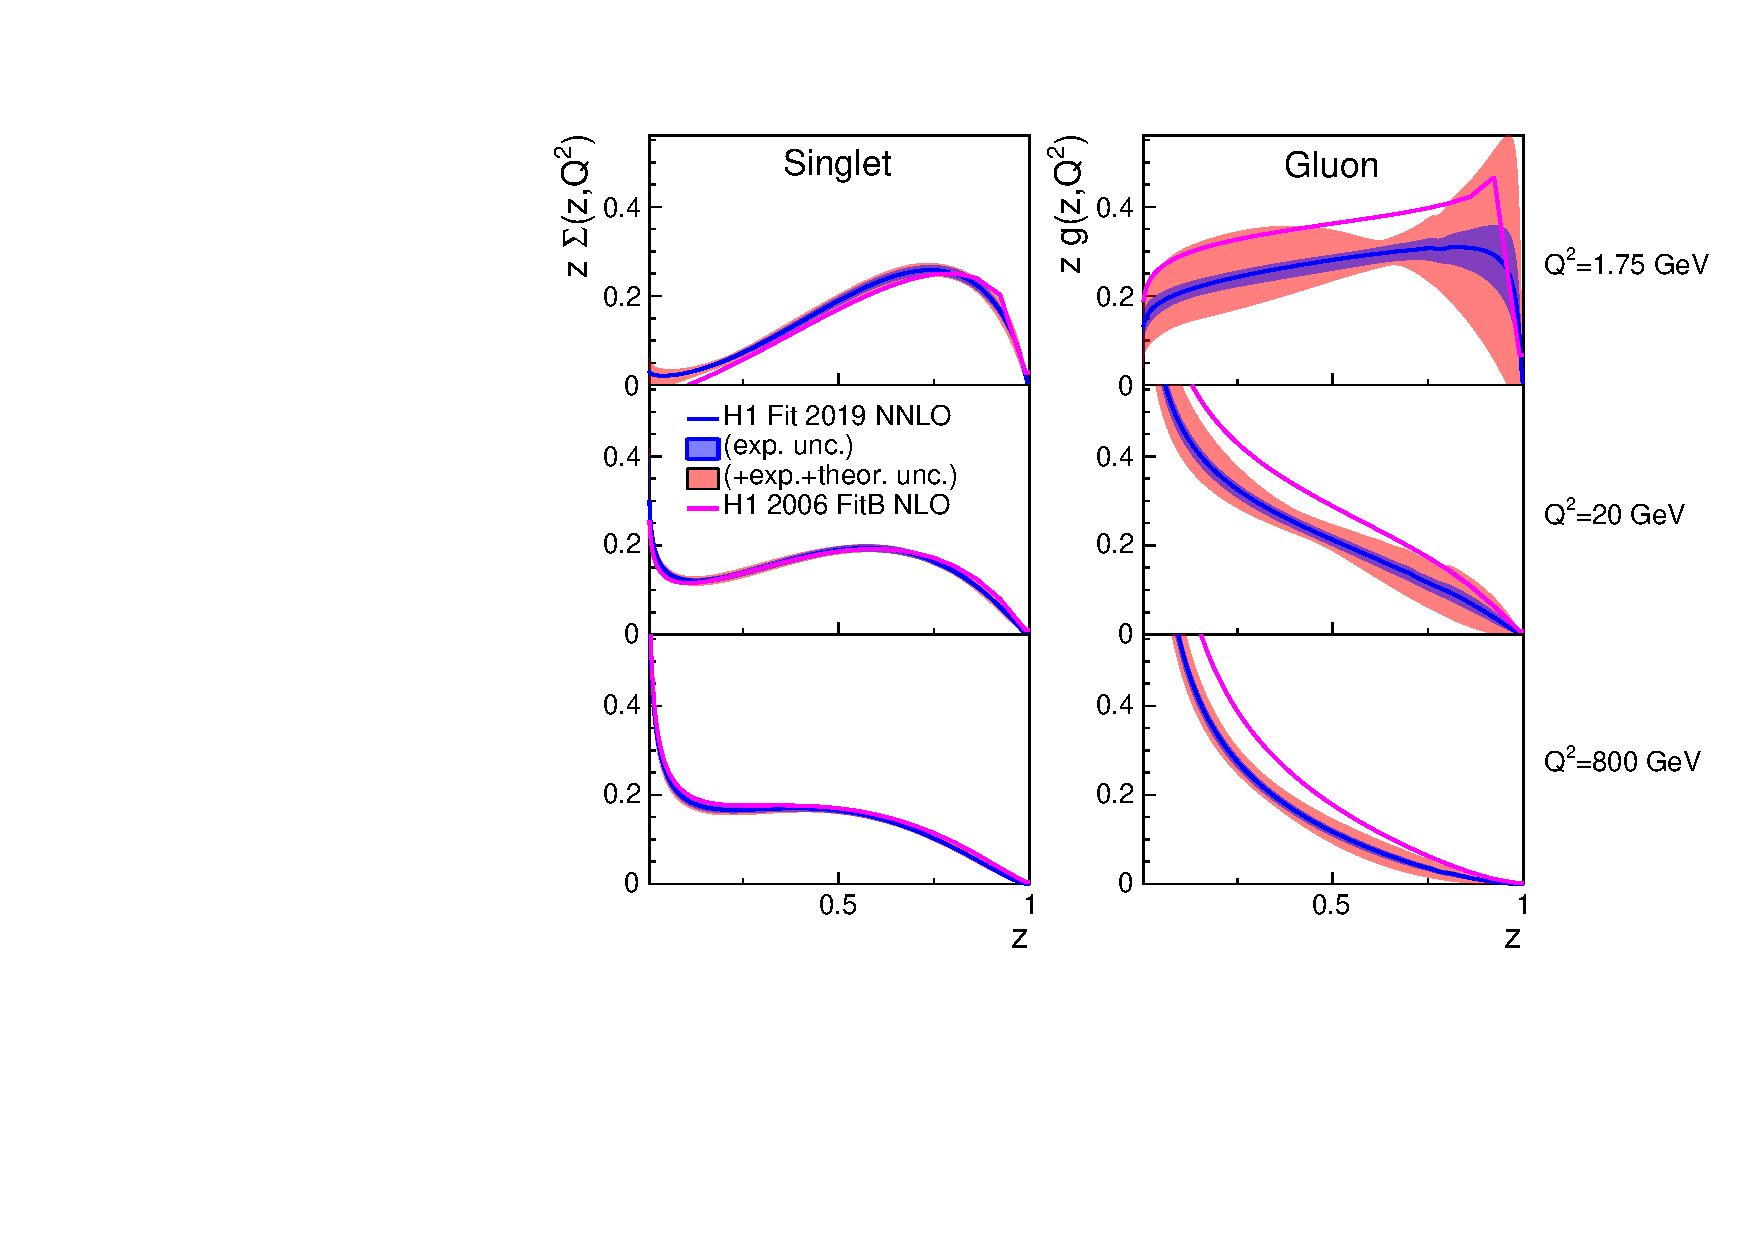
\includegraphics[width=0.9\textwidth]{{{plots/pdfsLin}.pdf}}
\end{center}
\caption{
  Singlet (left, $\Sigma$) and gluon (right, $g$) distributions of the pomeron
  in \DPDF as a function of $z$
  for three different values of \muf\ at a value of $\xpom=0.003$.
  The inner (dark) error band displays the experimental uncertainty, while
  the outer (bright) error band displays the full uncertainty, i.e.\ experimental,
  parameterisation, model and theoretical uncertainties added in quadrature.
  The \DPDF is compared to \DPDFFitB\ (dashed line), which was obtained in an NLO pQCD fit.
}
\label{fig:pdfsLin}
\end{figure}

\begin{figure}[tbhp]
\begin{center}
  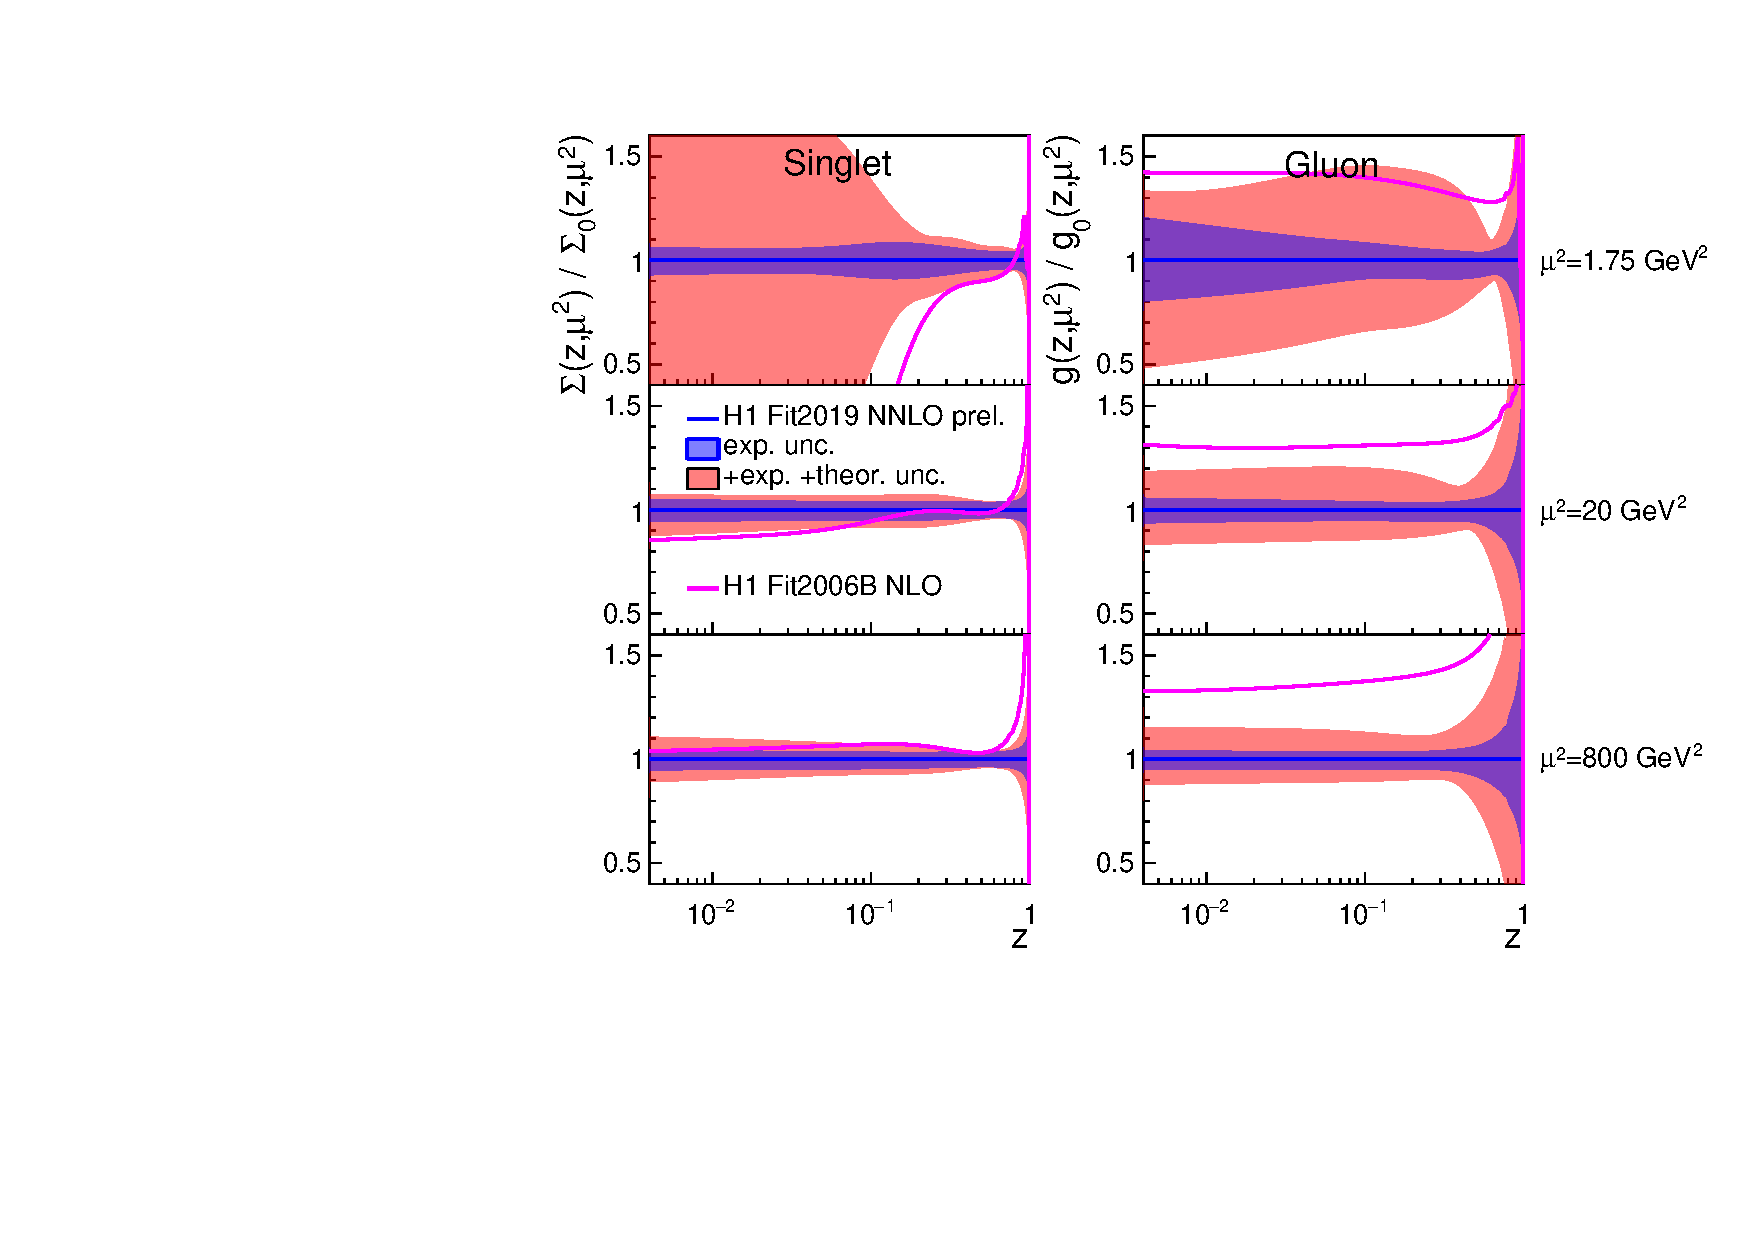
\includegraphics[width=0.9\textwidth]{{{plots/pdfsRatLog}.pdf}}
\end{center}
\caption{
  Ratio to \DPDF\ as function of $z$for three different values
  of \muf\ at a value of $\xpom=0.003$.
  More details as in fig.~\ref{fig:pdfsLin}.
  Mind the logarithmic scale of the abscissa in contrast to fig.~\ref{fig:pdfsLin}.
}
\label{fig:pdfsRatLog}
\end{figure}


\begin{figure}[tbhp]
\begin{center}
  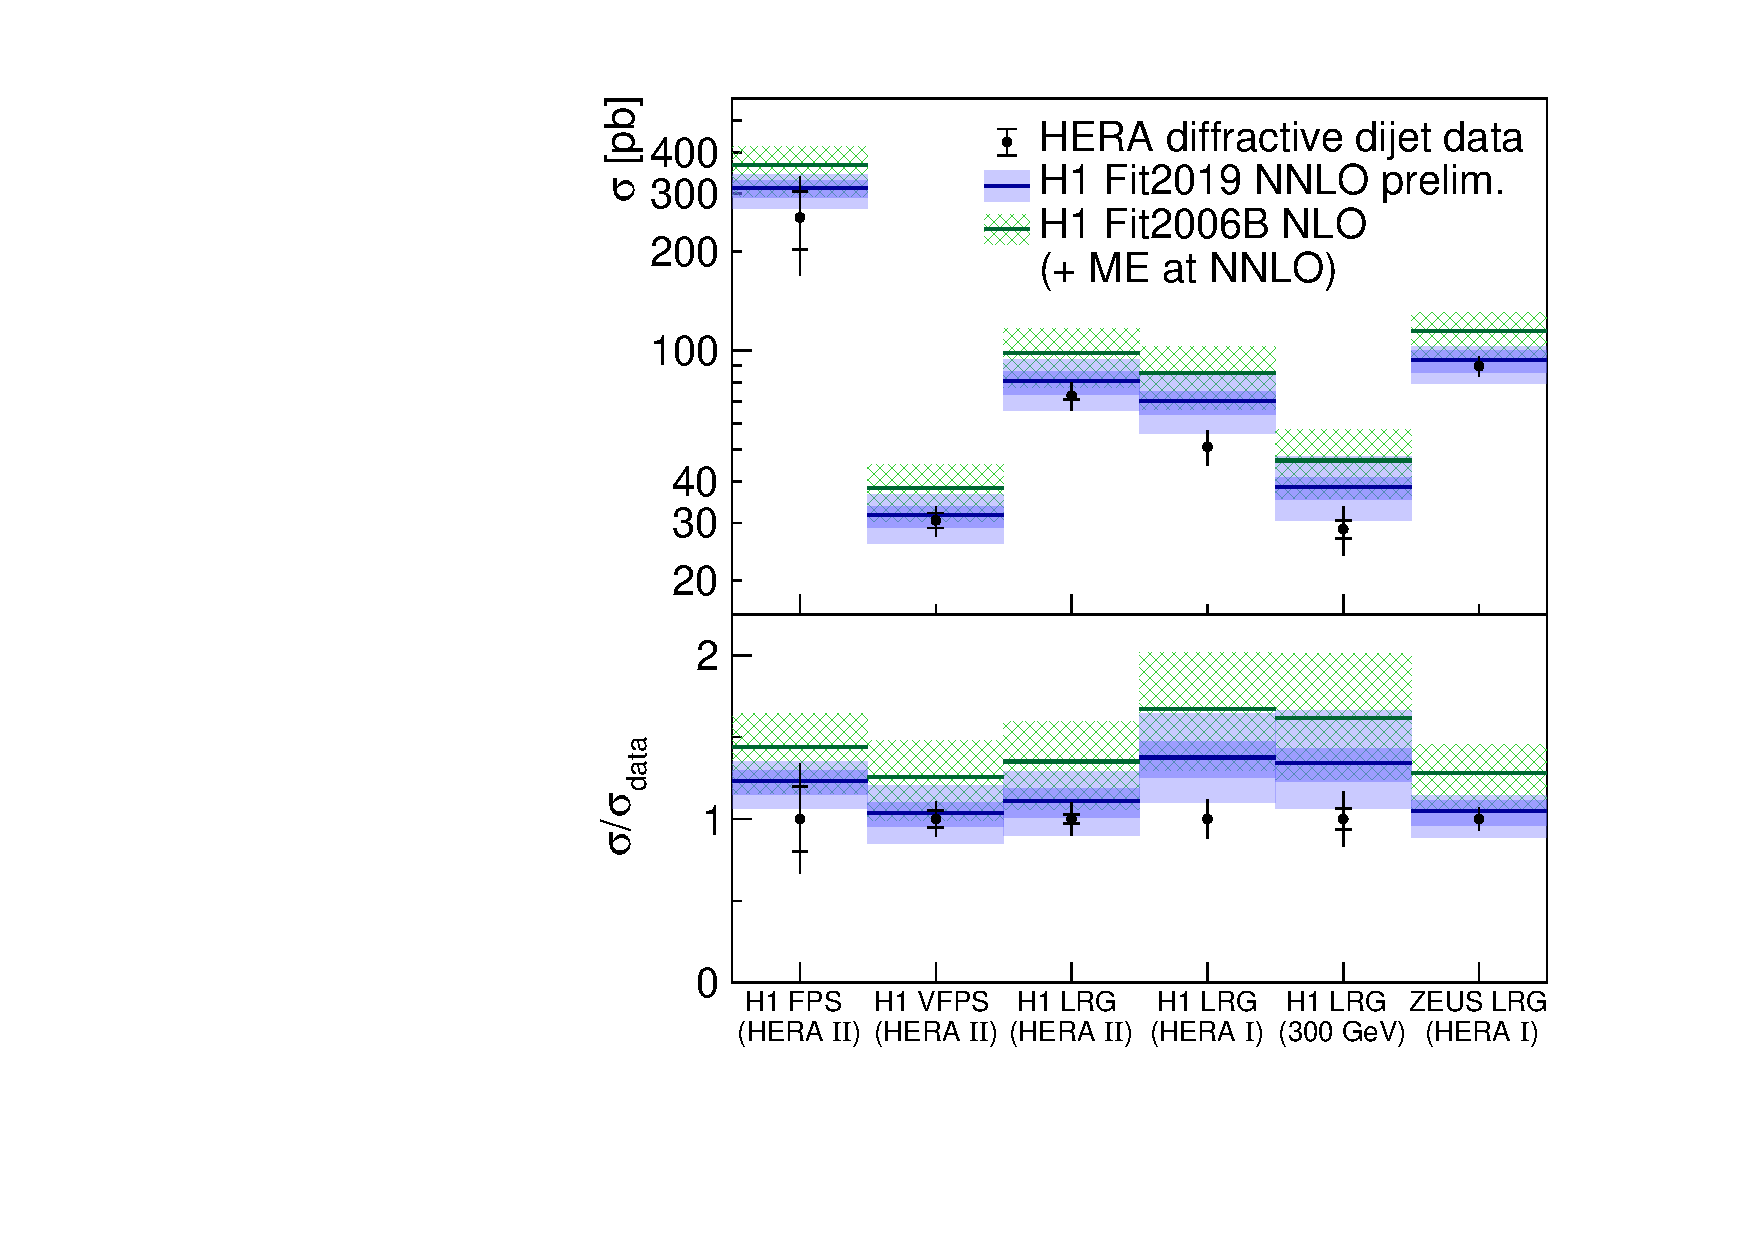
\includegraphics[width=0.8\textwidth]{{{plots/total}.pdf}}
\end{center}
\caption{
  NNLO pQCD predictions (full blue line) using \DPDF\ in comparison to the total dijet cross section measured in six different
  analysis by the H1 or ZEUS collaborations (full circles).
  For comparison, also NLO pQCD predictions using \DPDFFitB\ are displayed.
  The upper panel displays the total cross section, and the lower panel the ratio
  of the predictions to data.
  The inner error band (dark blue) displays the DPDF uncertainty of the \DPDF\ fit,
  and the outer error band (light blue) displays the DPDF uncertainty and scale
  uncertainty added in quadrature.
  The hatched band displays the DPDF uncertainty and NLO scale uncertainty of the NLO predictions.
  The inner error of the data displays the statistical uncertainty, and the full error bars displays the total experimental uncertainty.
}
\label{fig:jets}
\end{figure}



\begin{figure}[tbhp]
\begin{center}
     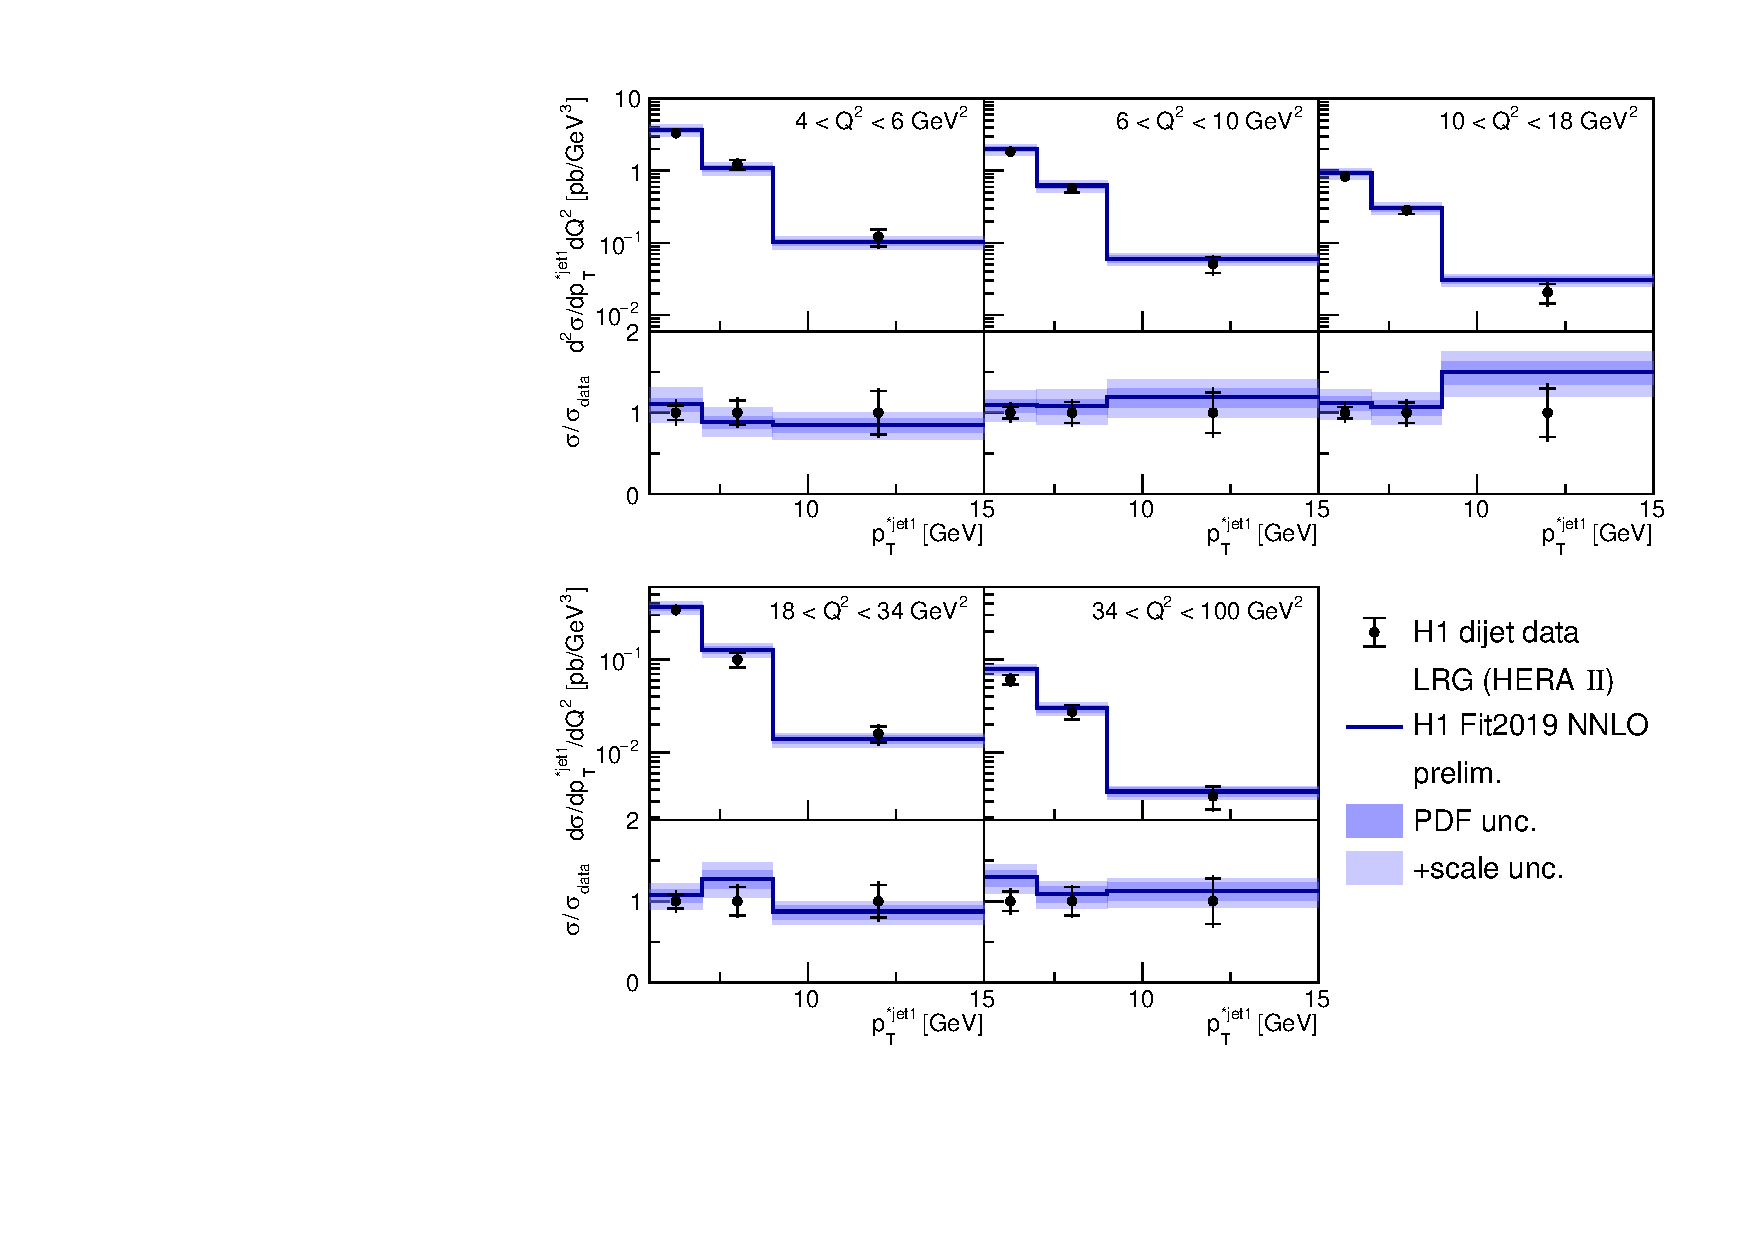
\includegraphics[width=0.94\textwidth]{{plots/LRG_heraII_2D}.pdf}
\end{center}
\caption{
  Comparison of NNLO predictions using \DPDF\ (full line) to H1 dijet cross section data (full circles)
  as a function of \meanpt\ for different \Qsq\ intervals.
  The inner band indicates the uncertainties associated to the \DPDF.
  The outer band incorporates the scale uncertainty.
}
\label{fig:}
\end{figure}


\begin{figure}[tbhp]
\begin{center}
     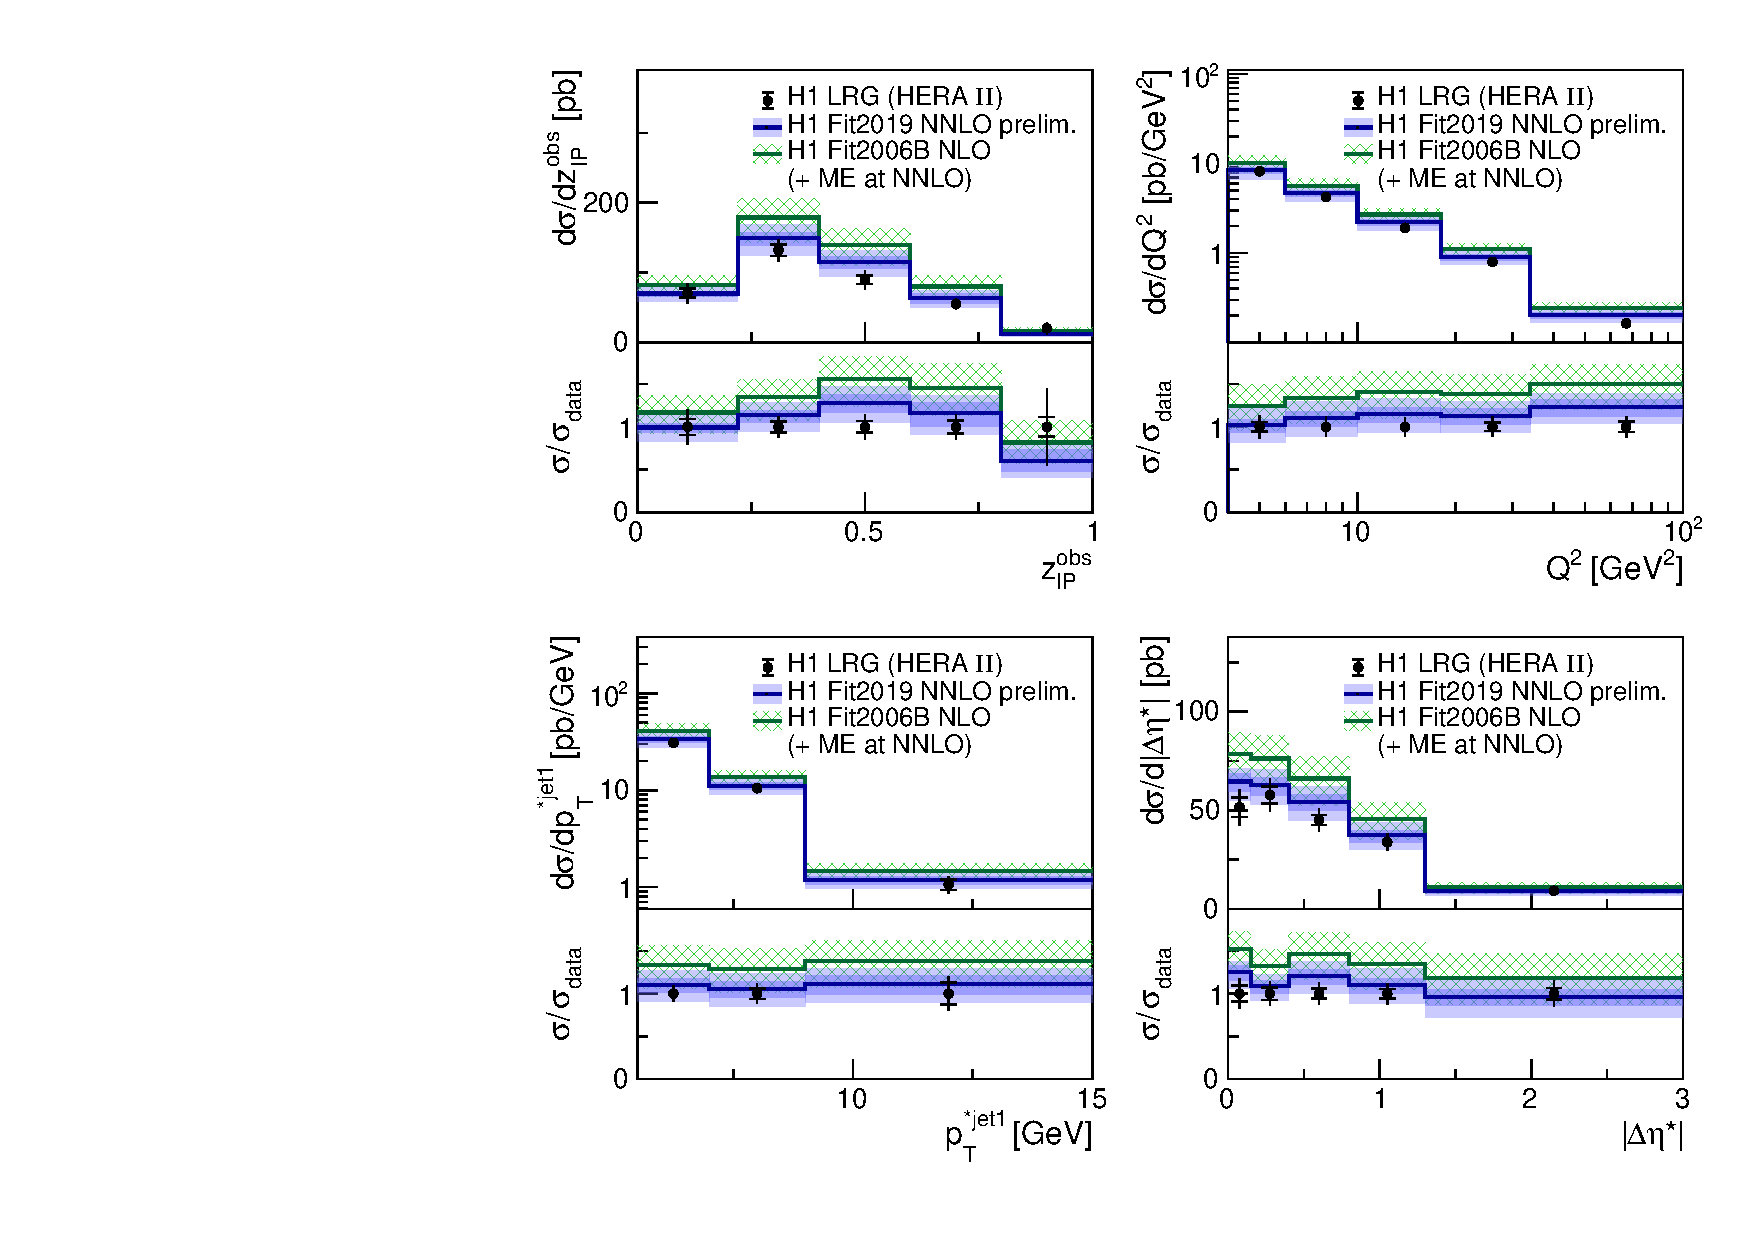
\includegraphics[width=0.84\textwidth]{{plots/LRG_heraII}.pdf}
\end{center}
\caption{
  Comparison of NNLO predictions using \DPDF\ (full line) to H1 dijet cross section data (full circles)
  as a function of .
  The inner band indicates the uncertainties associated to the \DPDF.
  The outer band incorporates the scale uncertainty.
}
\label{fig:}
\end{figure}


\begin{figure}[tbhp]
\begin{center}
     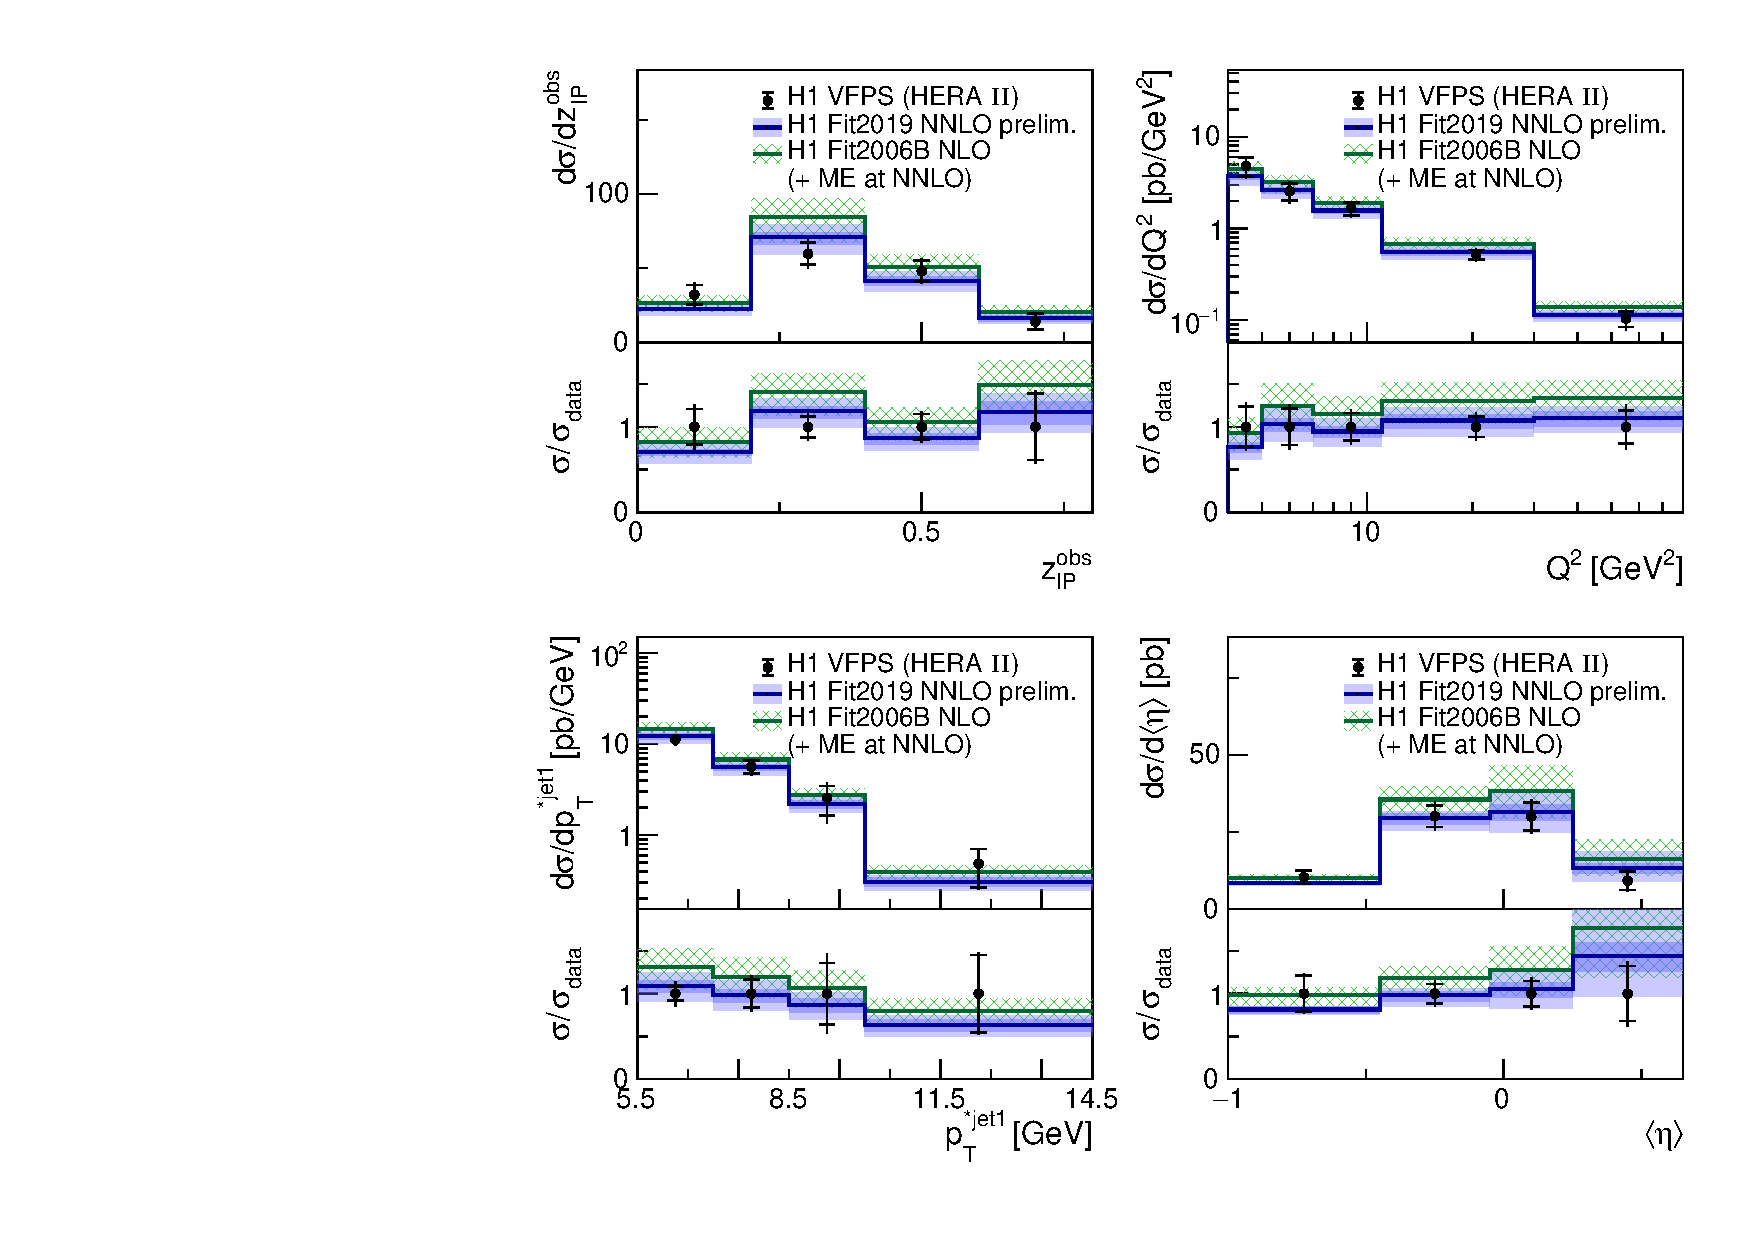
\includegraphics[width=0.84\textwidth]{{plots/VFPS}.pdf}
\end{center}
\caption{
  Comparison of NNLO predictions using \DPDF\ (full line) to ZEUS dijet cross section data (full circles)
  as a function of .
  The inner band indicates the uncertainties associated to the \DPDF.
  The outer band incorporates the scale uncertainty.
}
\label{fig:}
\end{figure}


\begin{figure}[tbhp]
\begin{center}
     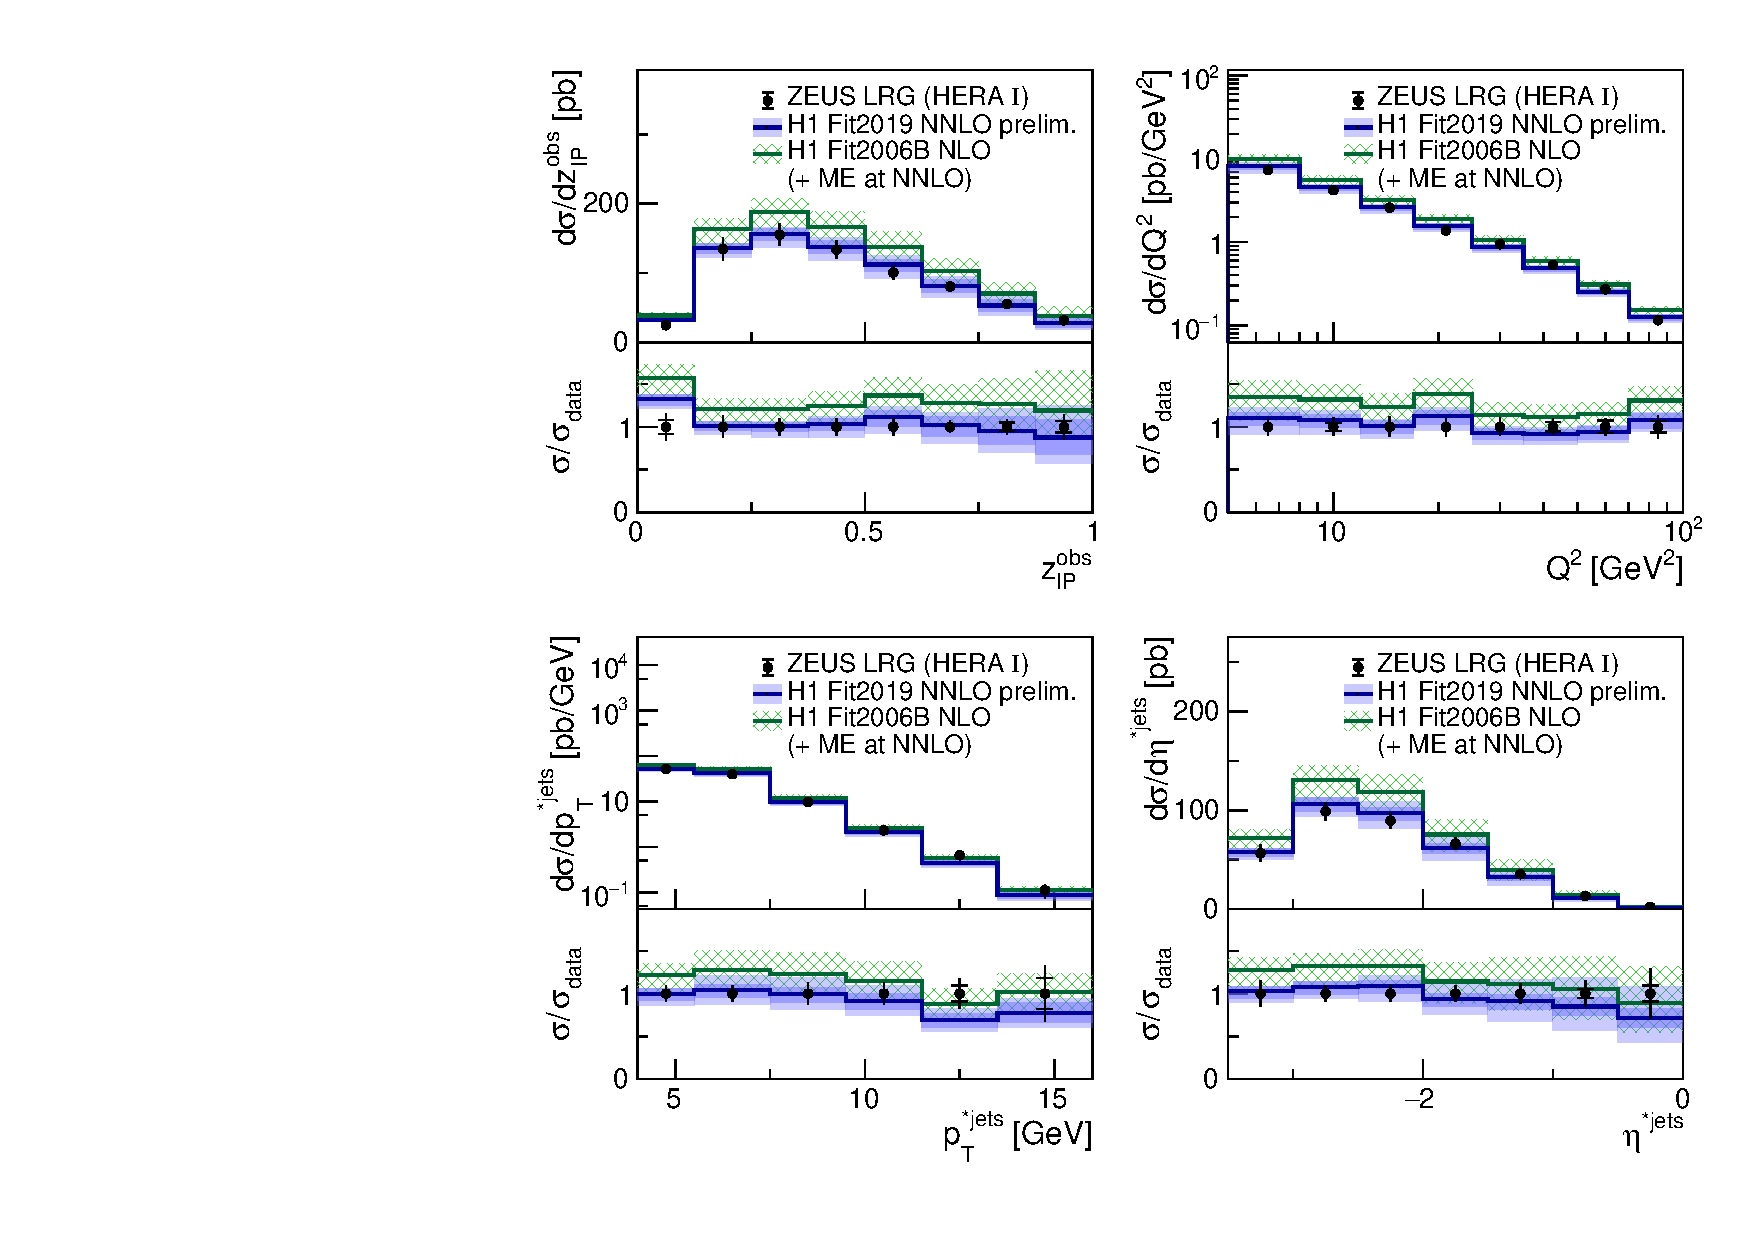
\includegraphics[width=0.84\textwidth]{{plots/LRG_ZEUS}.pdf}
\end{center}
\caption{
  Comparison of NNLO predictions using \DPDF\ (full line) to ZEUS dijet cross section data (full circles)
  as a function of .
  The inner band indicates the uncertainties associated to the \DPDF.
  The outer band incorporates the scale uncertainty.
}
\label{fig:}
\end{figure}





\begin{figure}[tbhp]
\begin{center}
  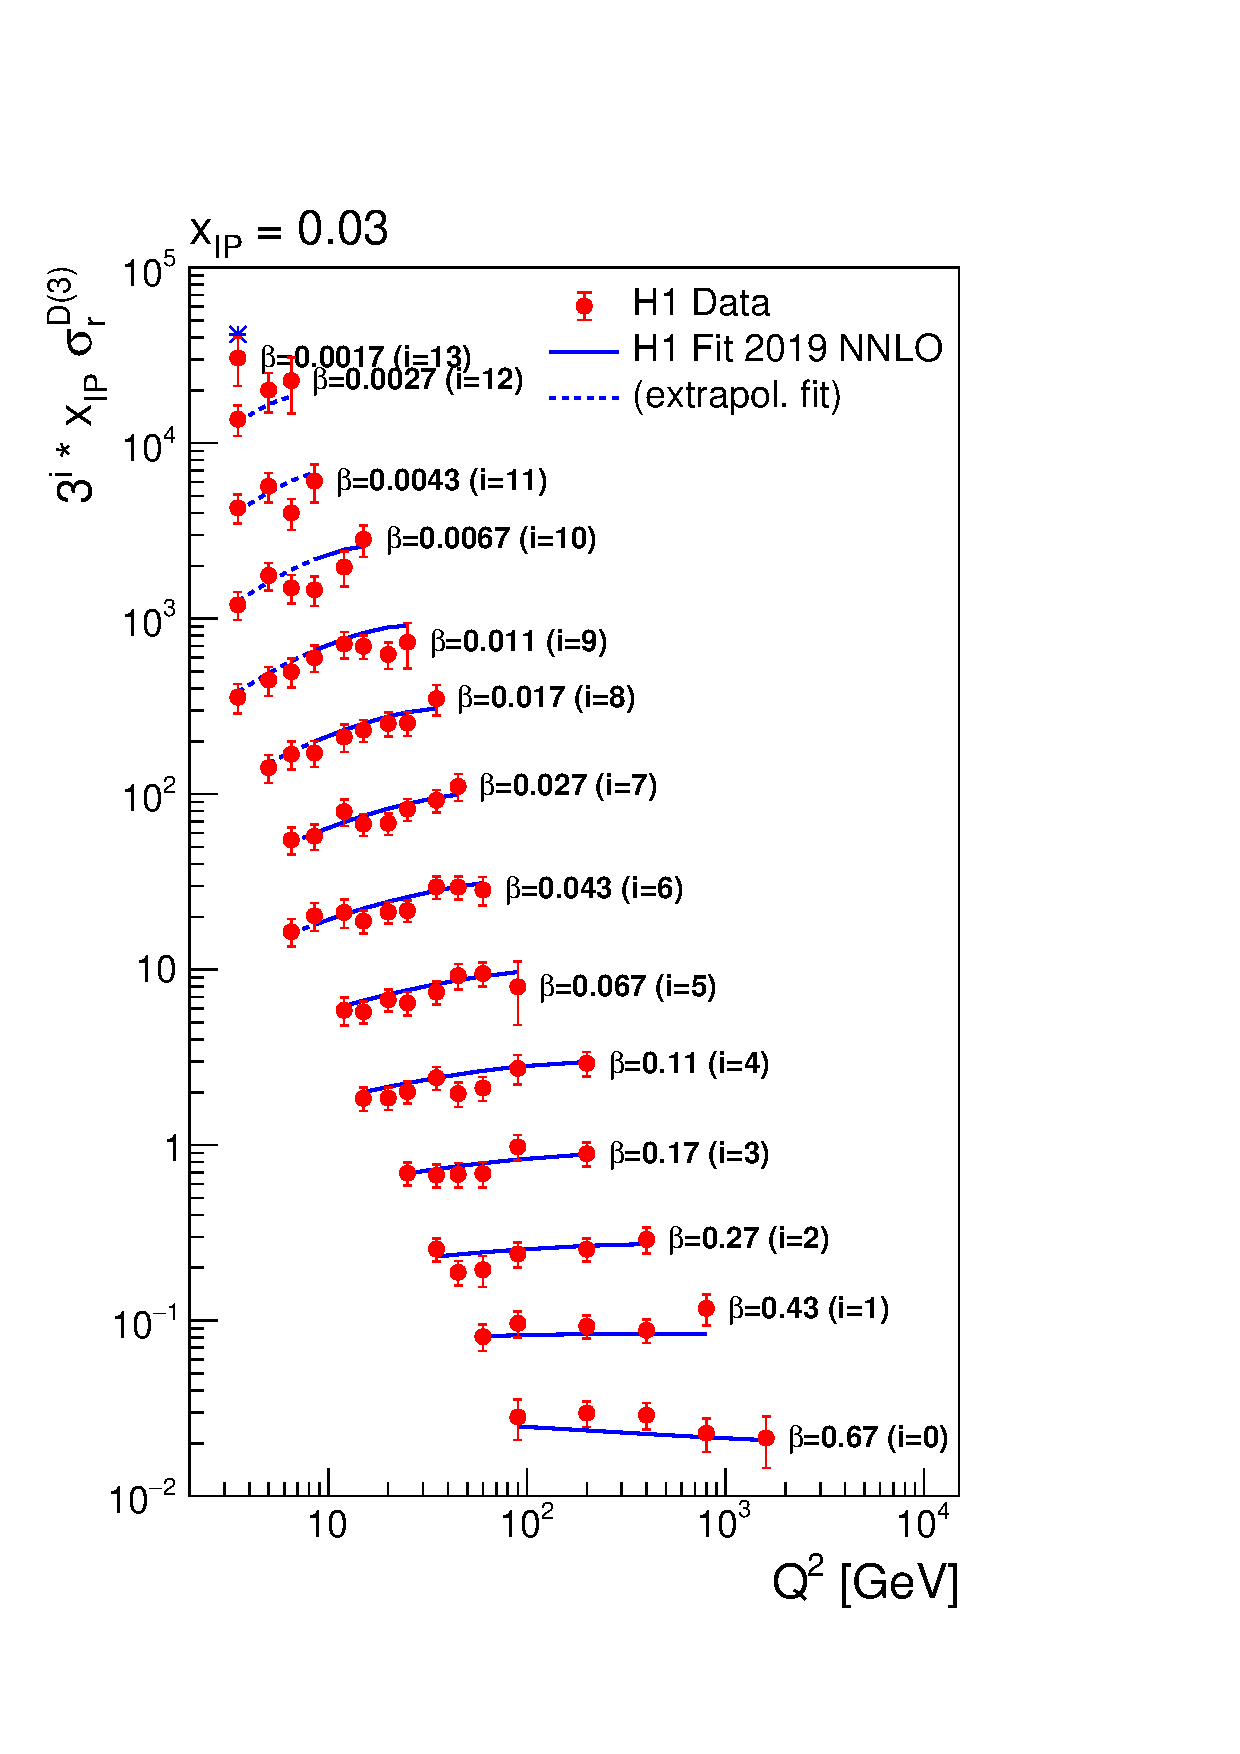
\includegraphics[width=0.7\textwidth]{{{plots/comb_q2_xpom0.03}.pdf}}
\end{center}
\caption{
  Comparison of (fitted) NNLO predictions using \DPDF\ (full line) to H1 combined LRG data at
  $\xpom=0.03$ (full circles) as a function of \Qsq.
  The predictions are extrapolated to data points, which are not included in the \DPDF fit (dashed line).
}
\label{fig:comb_q2_xpom0p03}
\end{figure}

\begin{figure}[tbhp]
\begin{center}
  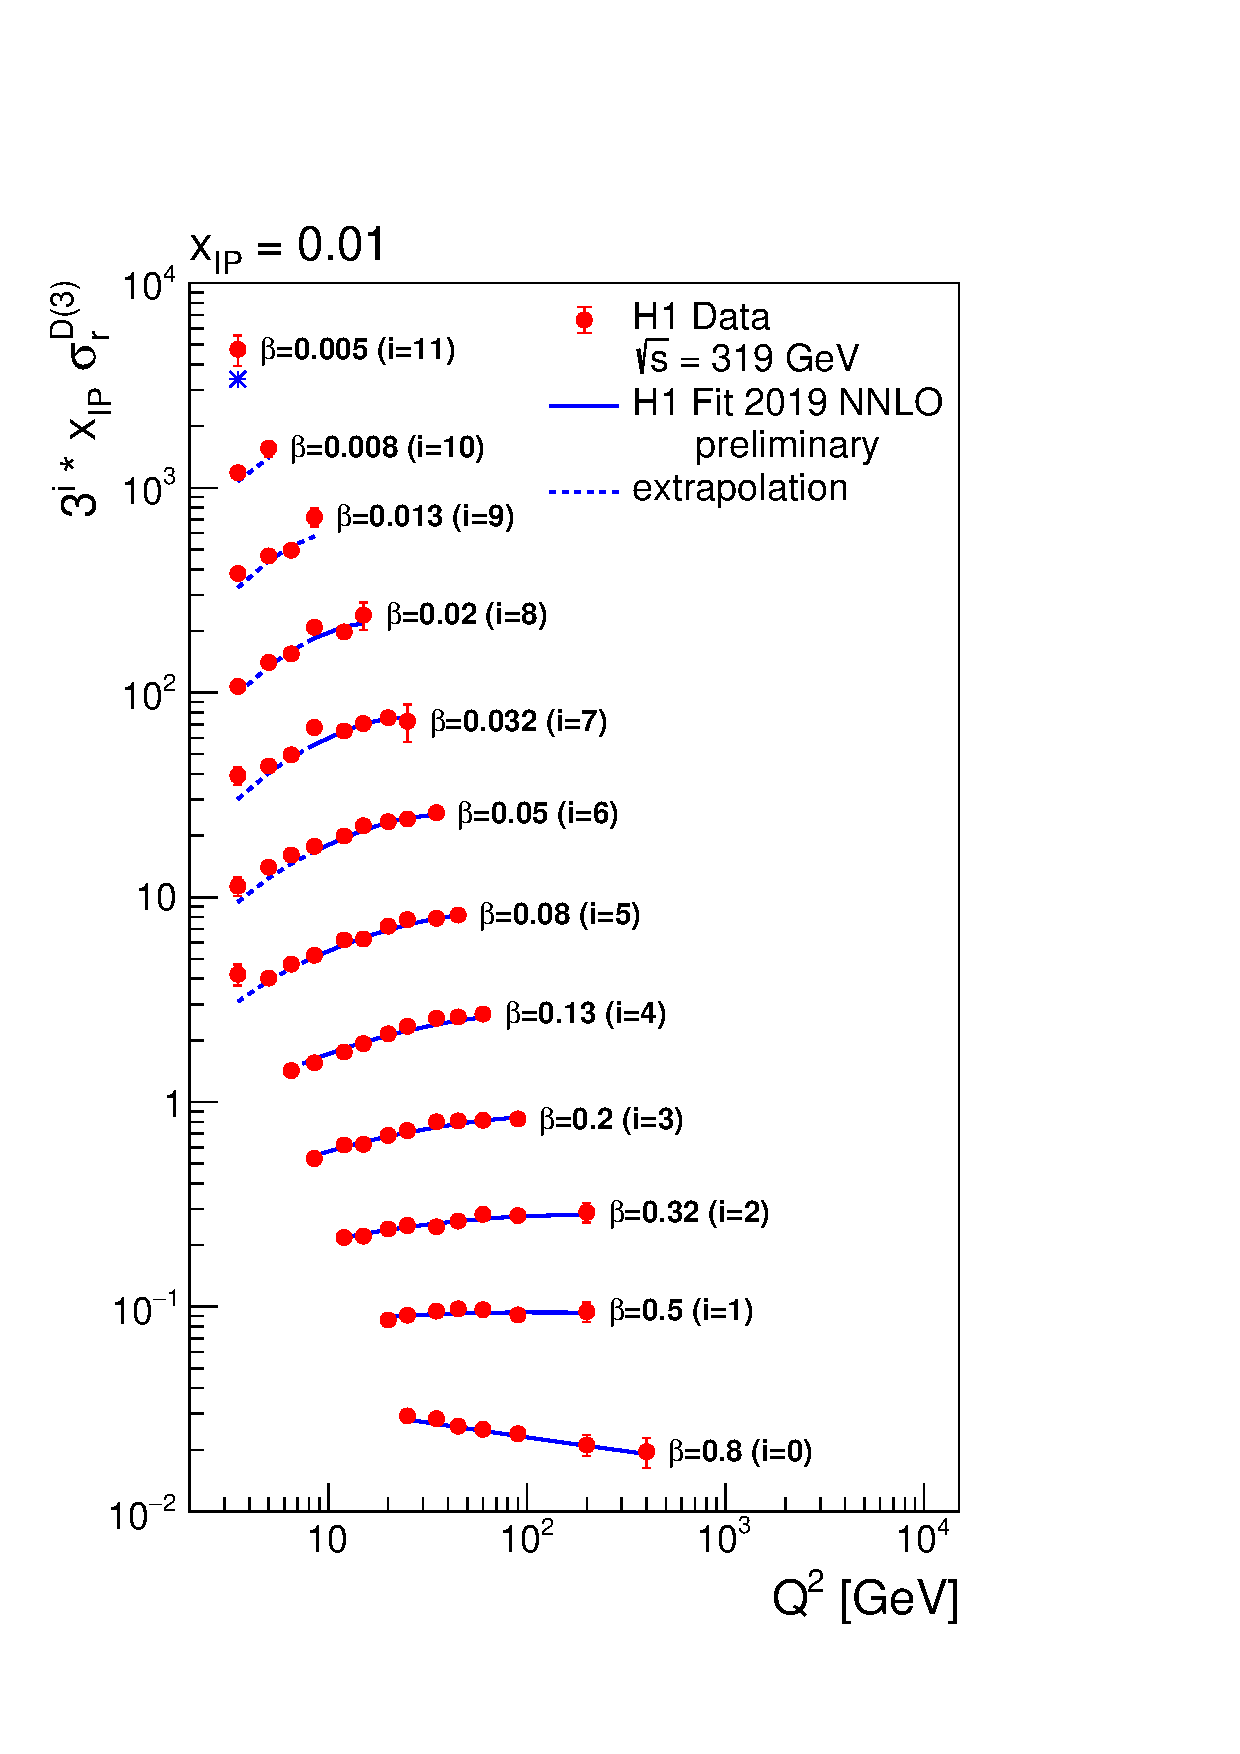
\includegraphics[width=0.7\textwidth]{{{plots/comb_q2_xpom0.01}.pdf}}
\end{center}
\caption{
  Comparison of (fitted) NNLO predictions using \DPDF\ (full line) to H1 combined LRG data as a function of \Qsq\ at
  $\xpom=0.01$ (full circles).
  Other details as in fig.~\ref{fig:comb_q2_xpom0p03}.
}
\label{fig:}
\end{figure}

\begin{figure}[tbhp]
\begin{center}
  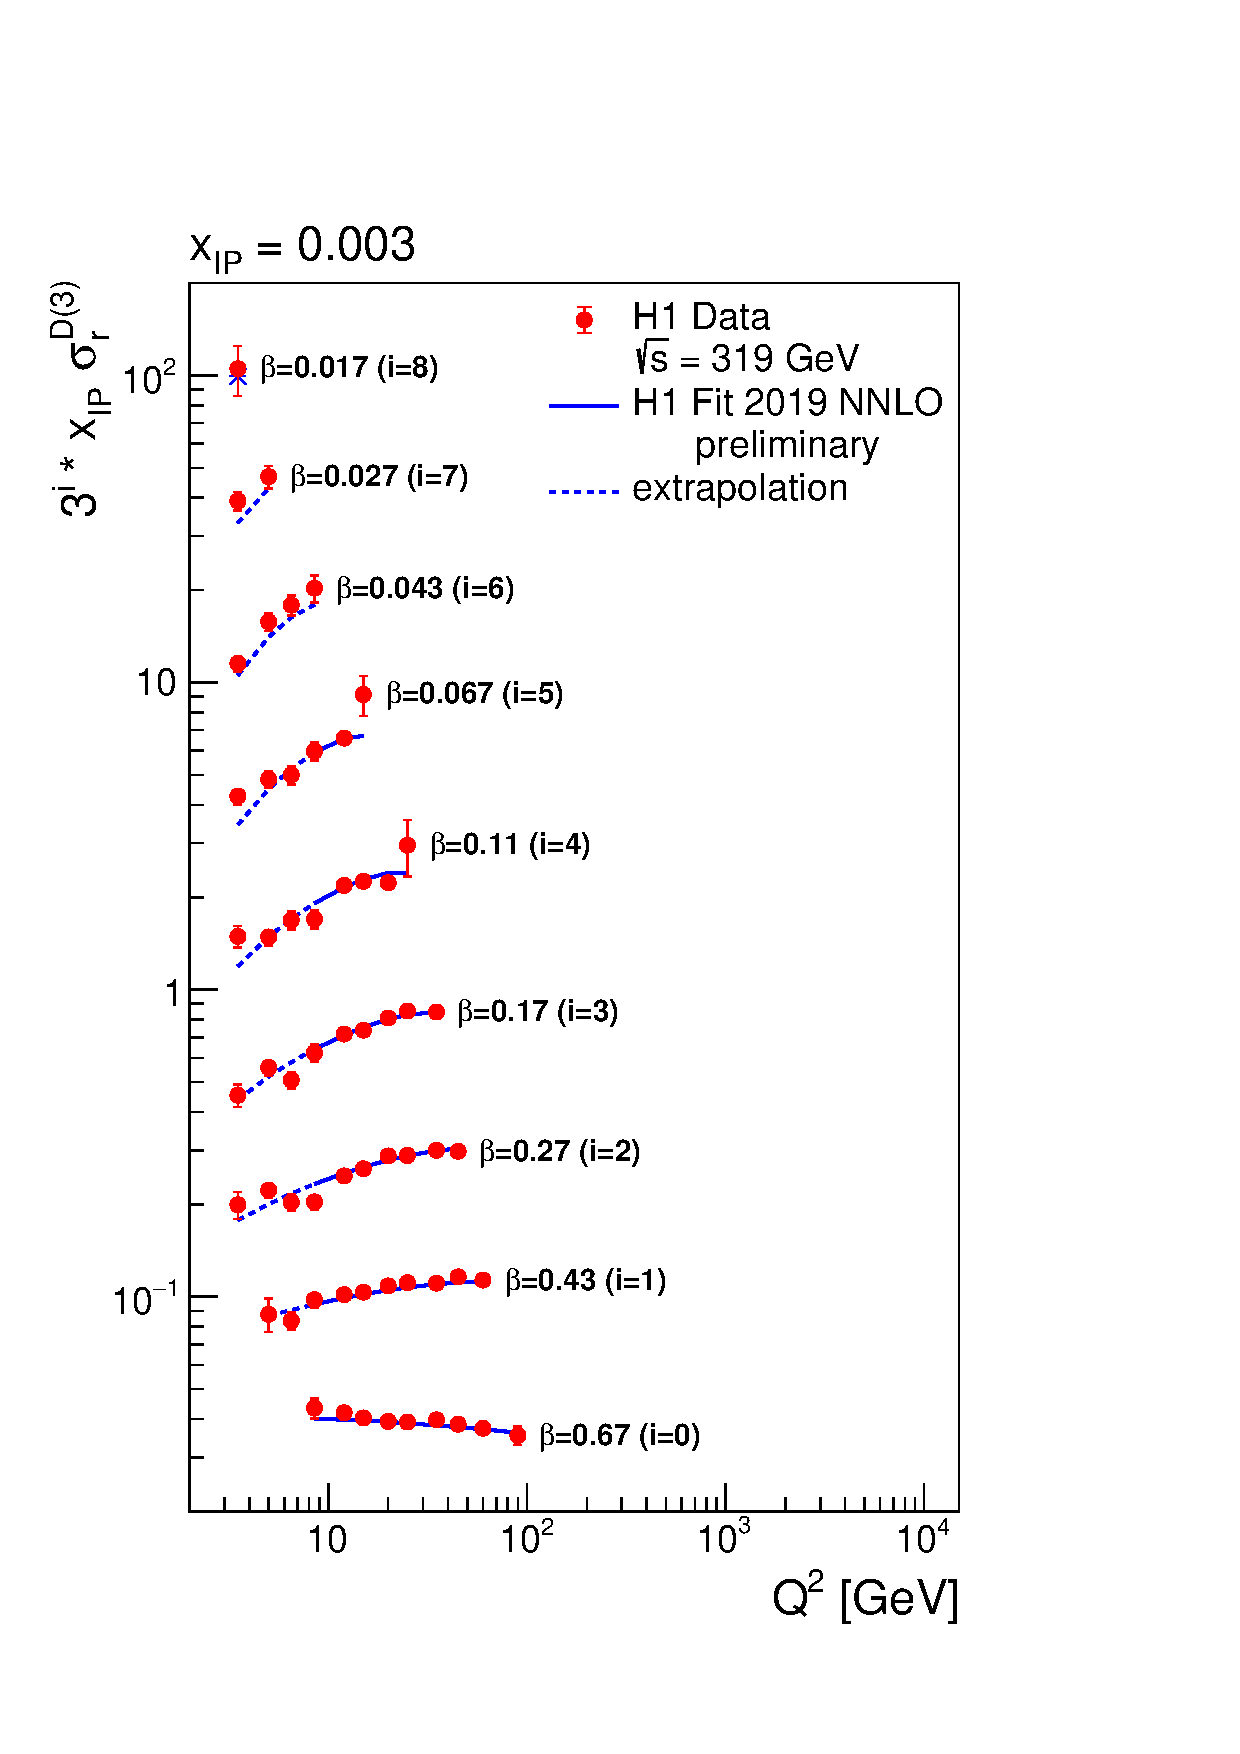
\includegraphics[width=0.7\textwidth]{{{plots/comb_q2_xpom0.003}.pdf}}
\end{center}
\caption{
  Comparison of (fitted) NNLO predictions using \DPDF\ (full line) to H1 combined LRG data as a function of \Qsq\ at
  $\xpom=0.003$ (full circles).
  Other details as in fig.~\ref{fig:comb_q2_xpom0p03}.
}
\label{fig:}
\end{figure}

\begin{figure}[tbhp]
\begin{center}
  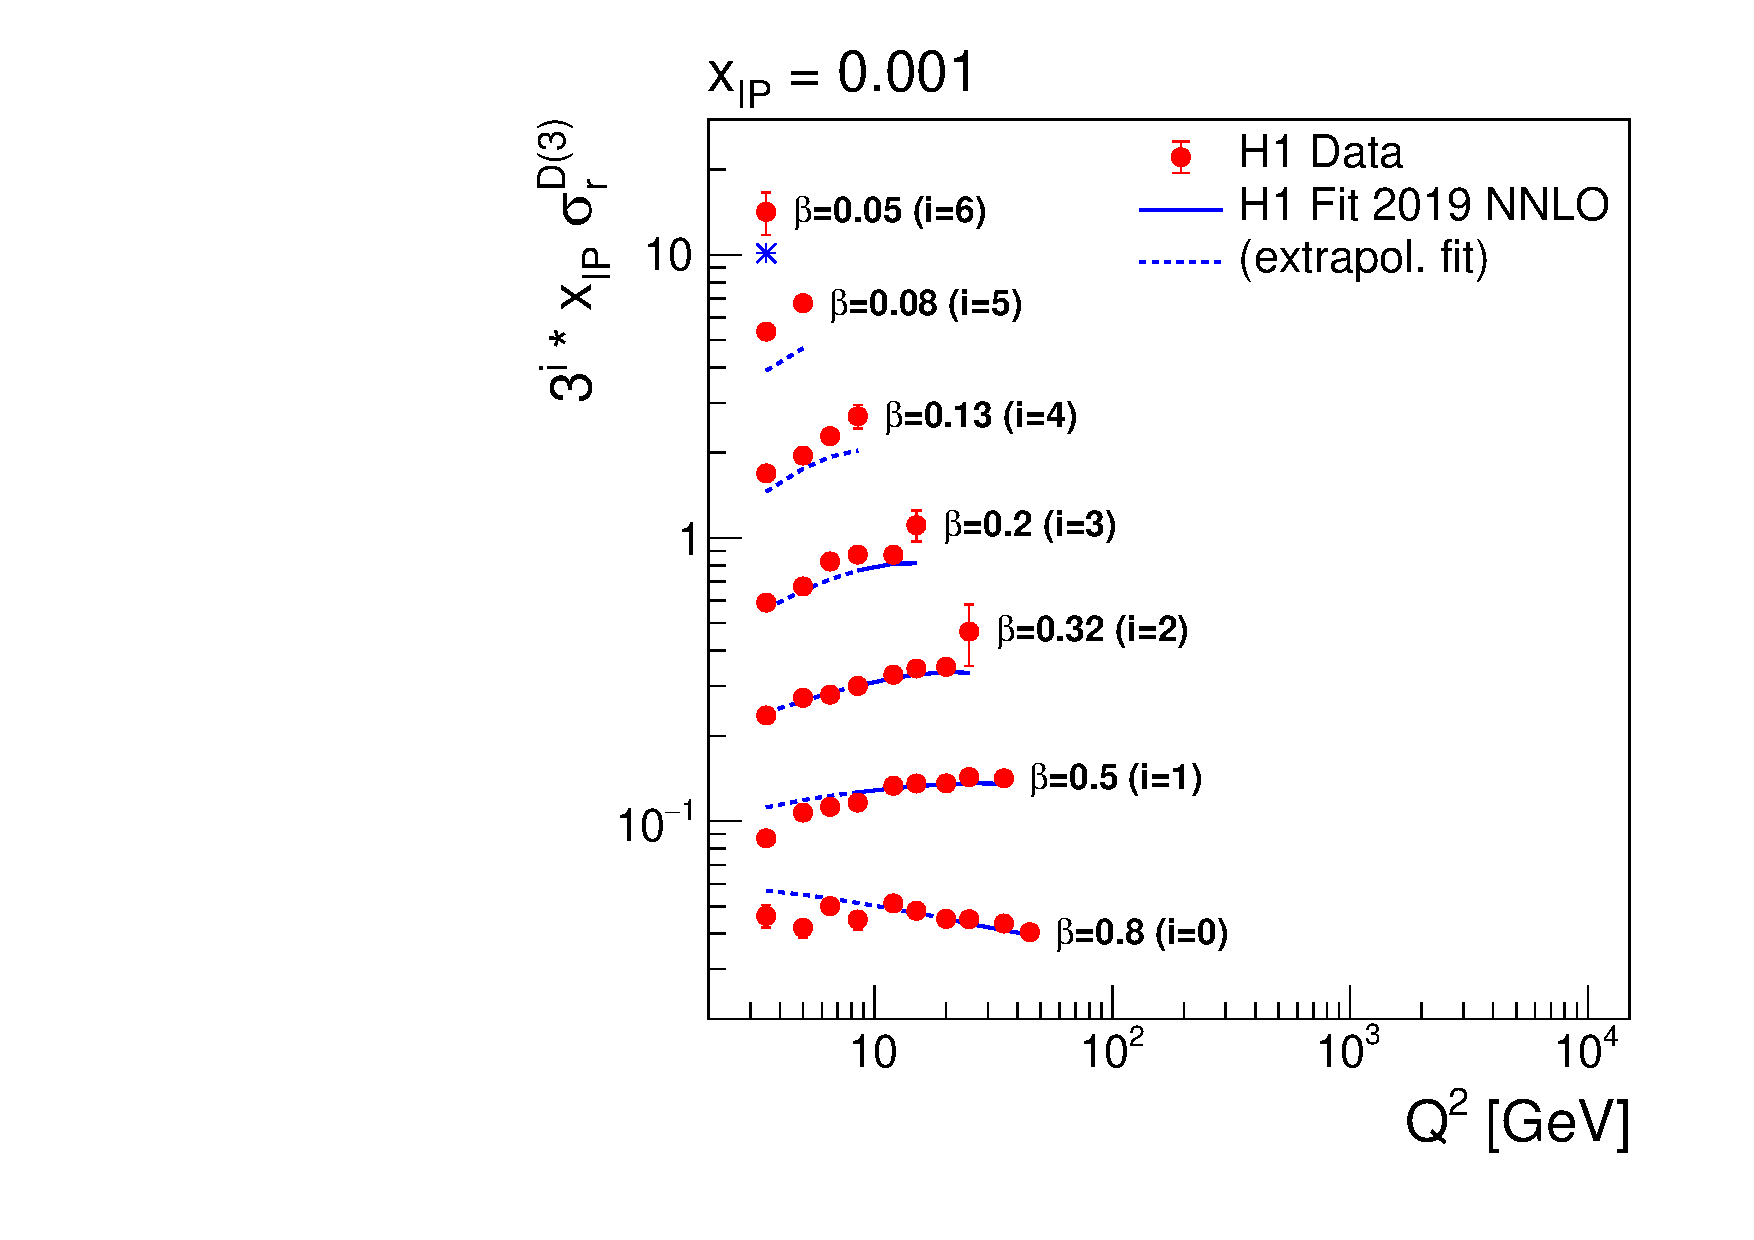
\includegraphics[width=0.7\textwidth]{{{plots/comb_q2_xpom0.001}.pdf}}
\end{center}
\caption{
  Comparison of (fitted) NNLO predictions using \DPDF\ (full line) to H1 combined LRG data as a function of \Qsq\ at
  $\xpom=0.001$ (full circles).
  Other details as in fig.~\ref{fig:comb_q2_xpom0p03}.
}
\label{fig:}
\end{figure}

\begin{figure}[tbhp]
\begin{center}
  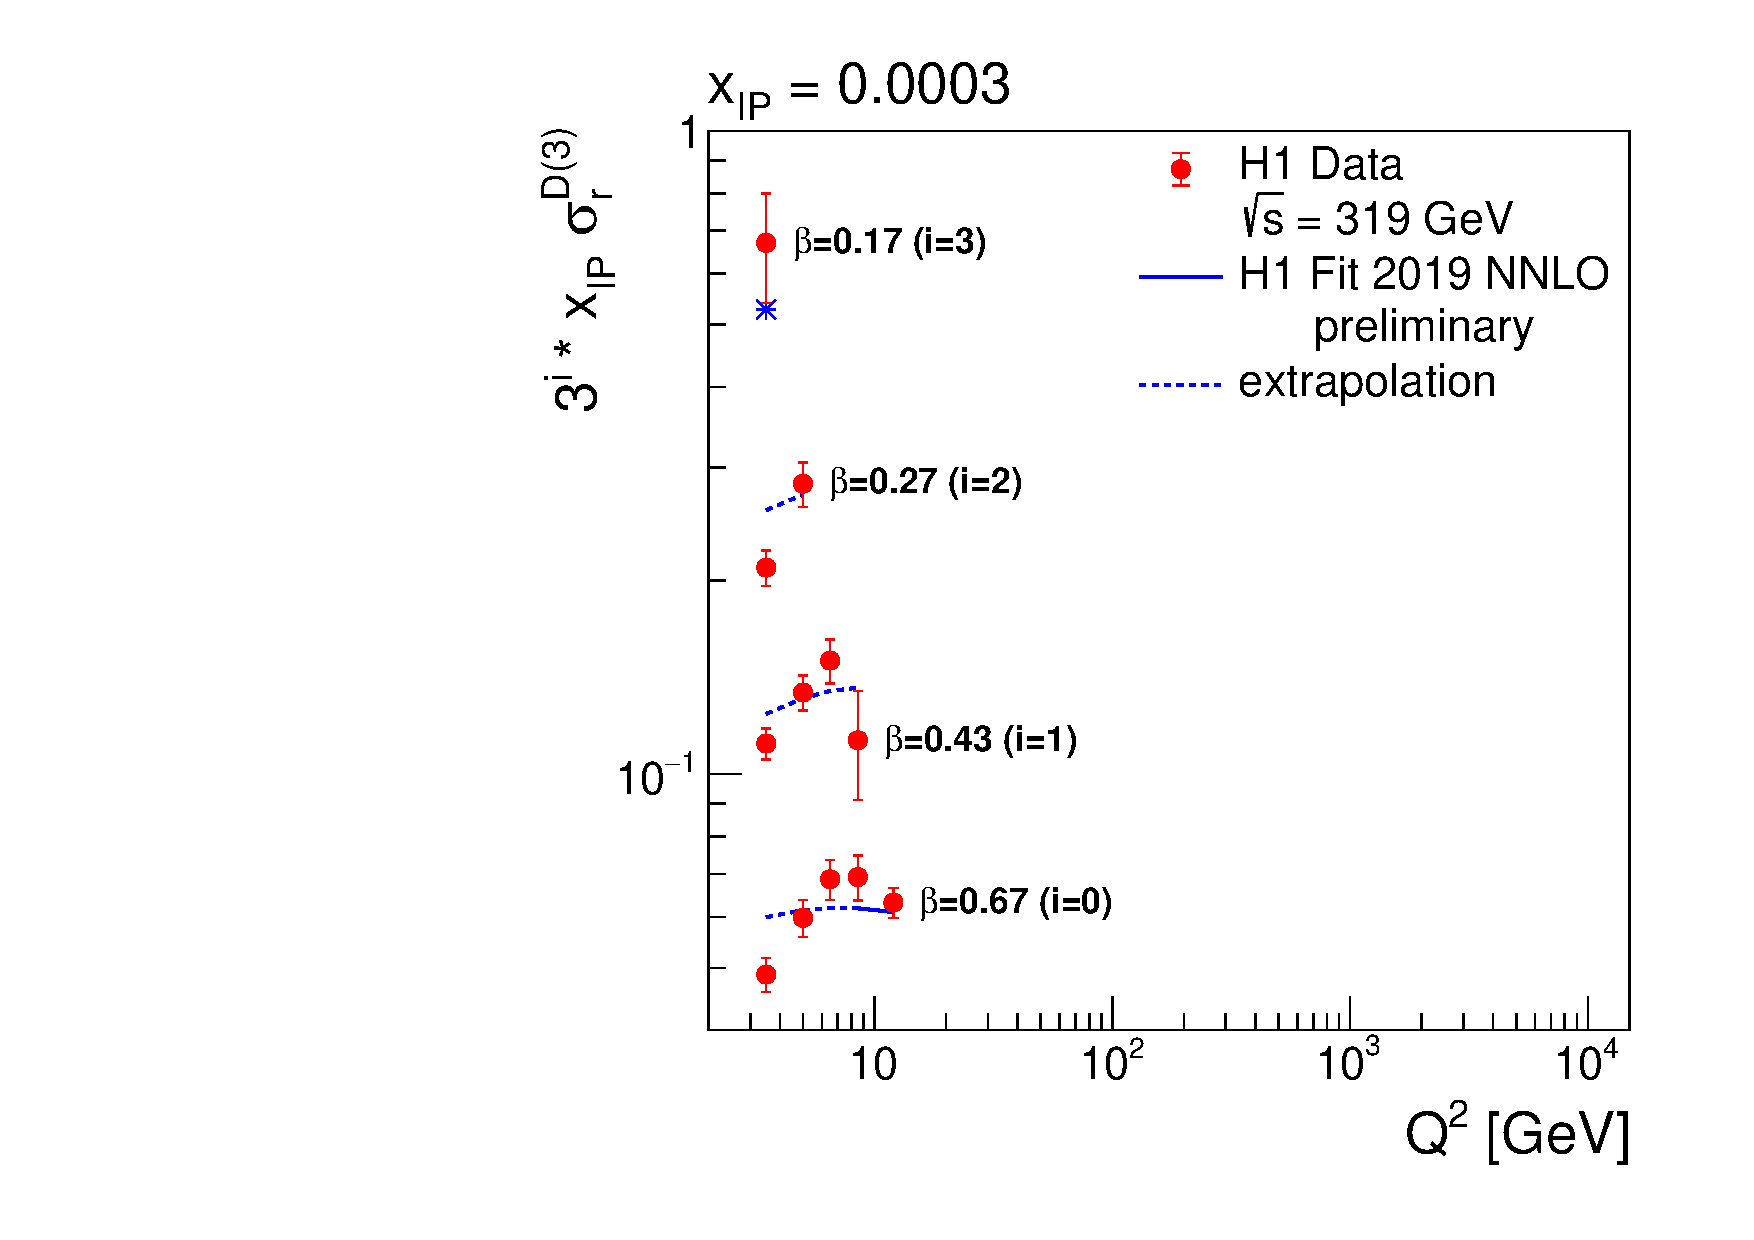
\includegraphics[width=0.7\textwidth]{{{plots/comb_q2_xpom0.0003}.pdf}}
\end{center}
\caption{
  Comparison of (fitted) NNLO predictions using \DPDF\ (full line) to H1 combined LRG data as a function of \Qsq\ at
  $\xpom=0.0003$ (full circles).
  Other details as in fig.~\ref{fig:comb_q2_xpom0p03}.
}
\label{fig:}
\end{figure}

\begin{figure}[tbhp]
\begin{center}
  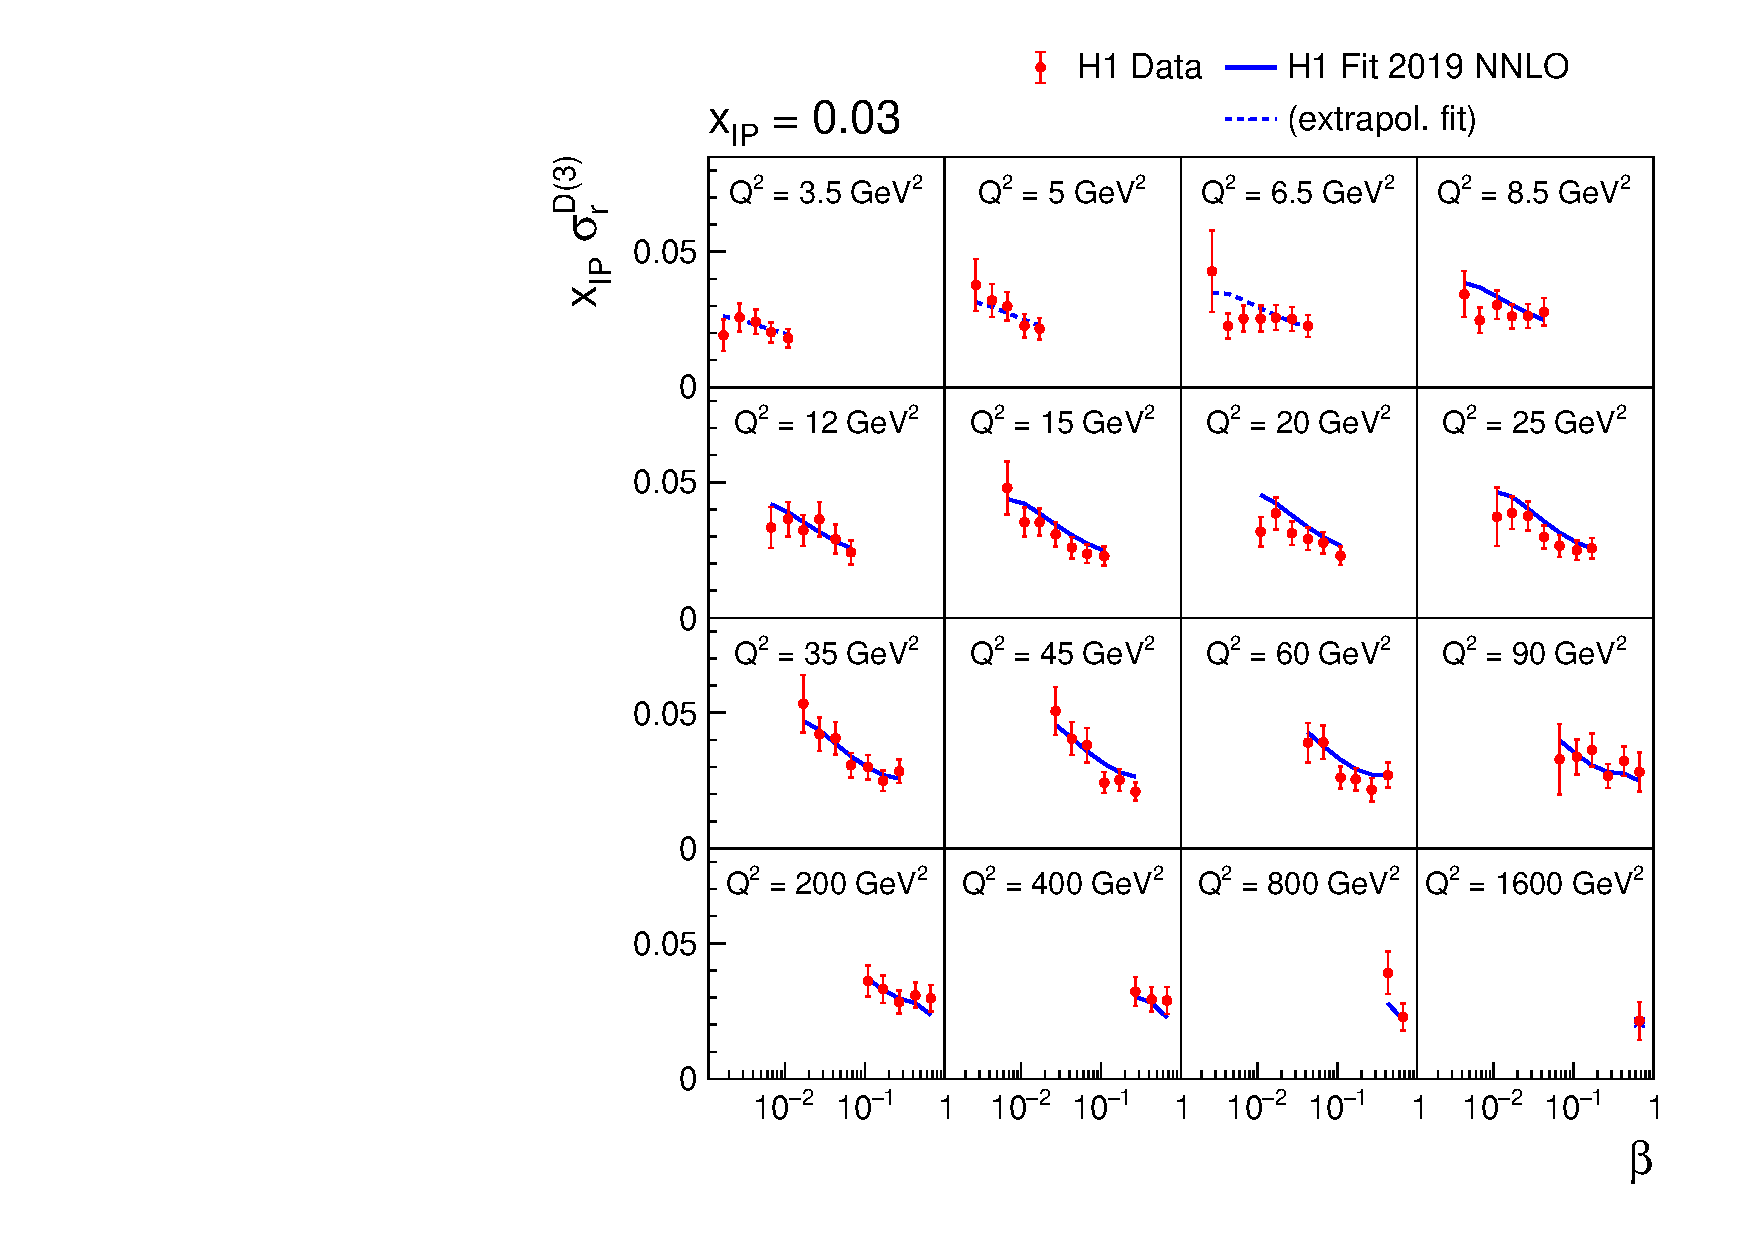
\includegraphics[width=0.8\textwidth]{{{plots/comb_beta_xpom0.03}.pdf}}
\end{center}
\caption{
  Comparison of (fitted) NNLO predictions using \DPDF\ (full line) to H1 combined LRG data as a function of $\beta$ at
  $\xpom=0.03$ (full circles).
  Other details as in fig.~\ref{fig:comb_q2_xpom0p03}.
}
\label{fig:}
\end{figure}

\begin{figure}[tbhp]
\begin{center}
  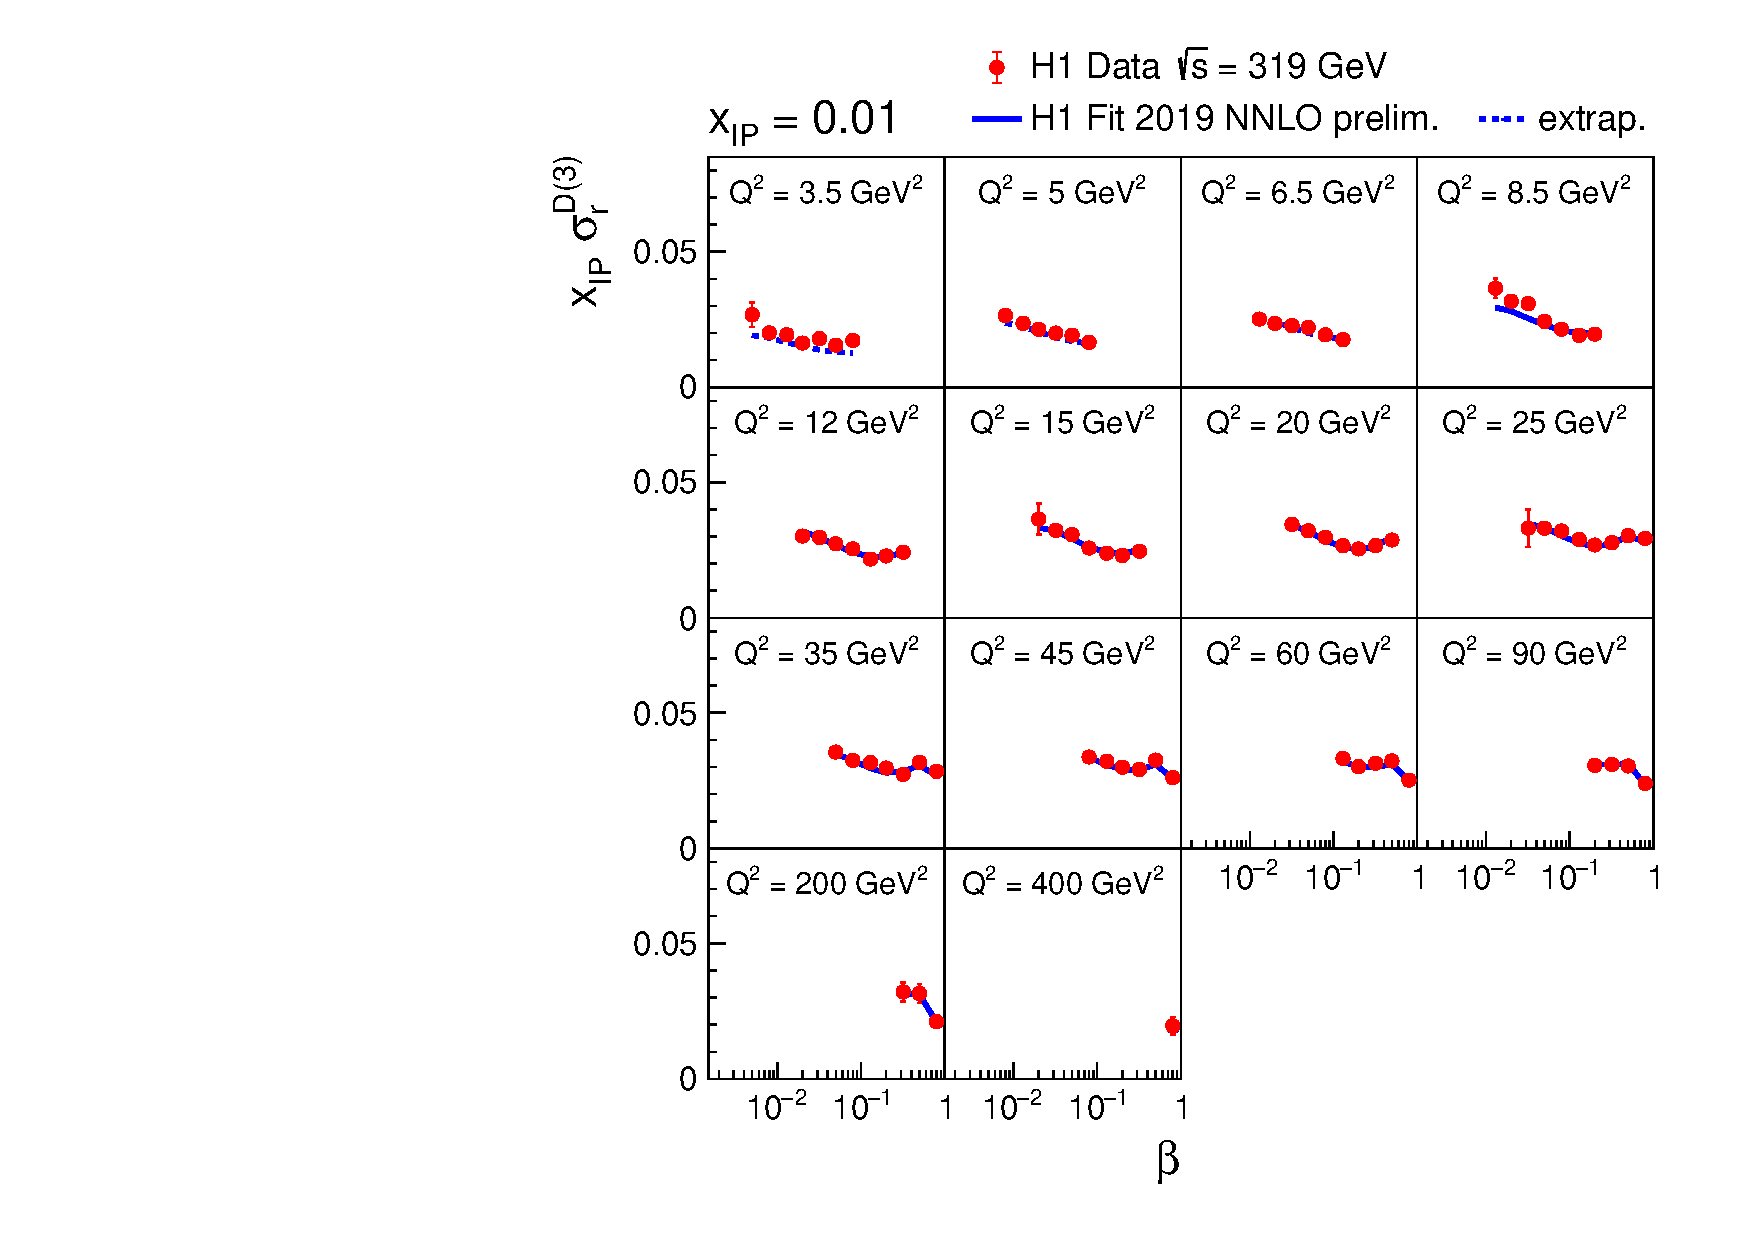
\includegraphics[width=0.8\textwidth]{{{plots/comb_beta_xpom0.01}.pdf}}
\end{center}
\caption{
  Comparison of (fitted) NNLO predictions using \DPDF\ (full line) to H1 combined LRG data as a function of $\beta$ at
  $\xpom=0.01$ (full circles).
  Other details as in fig.~\ref{fig:comb_q2_xpom0p03}.
}
\label{fig:}
\end{figure}

\begin{figure}[tbhp]
\begin{center}
  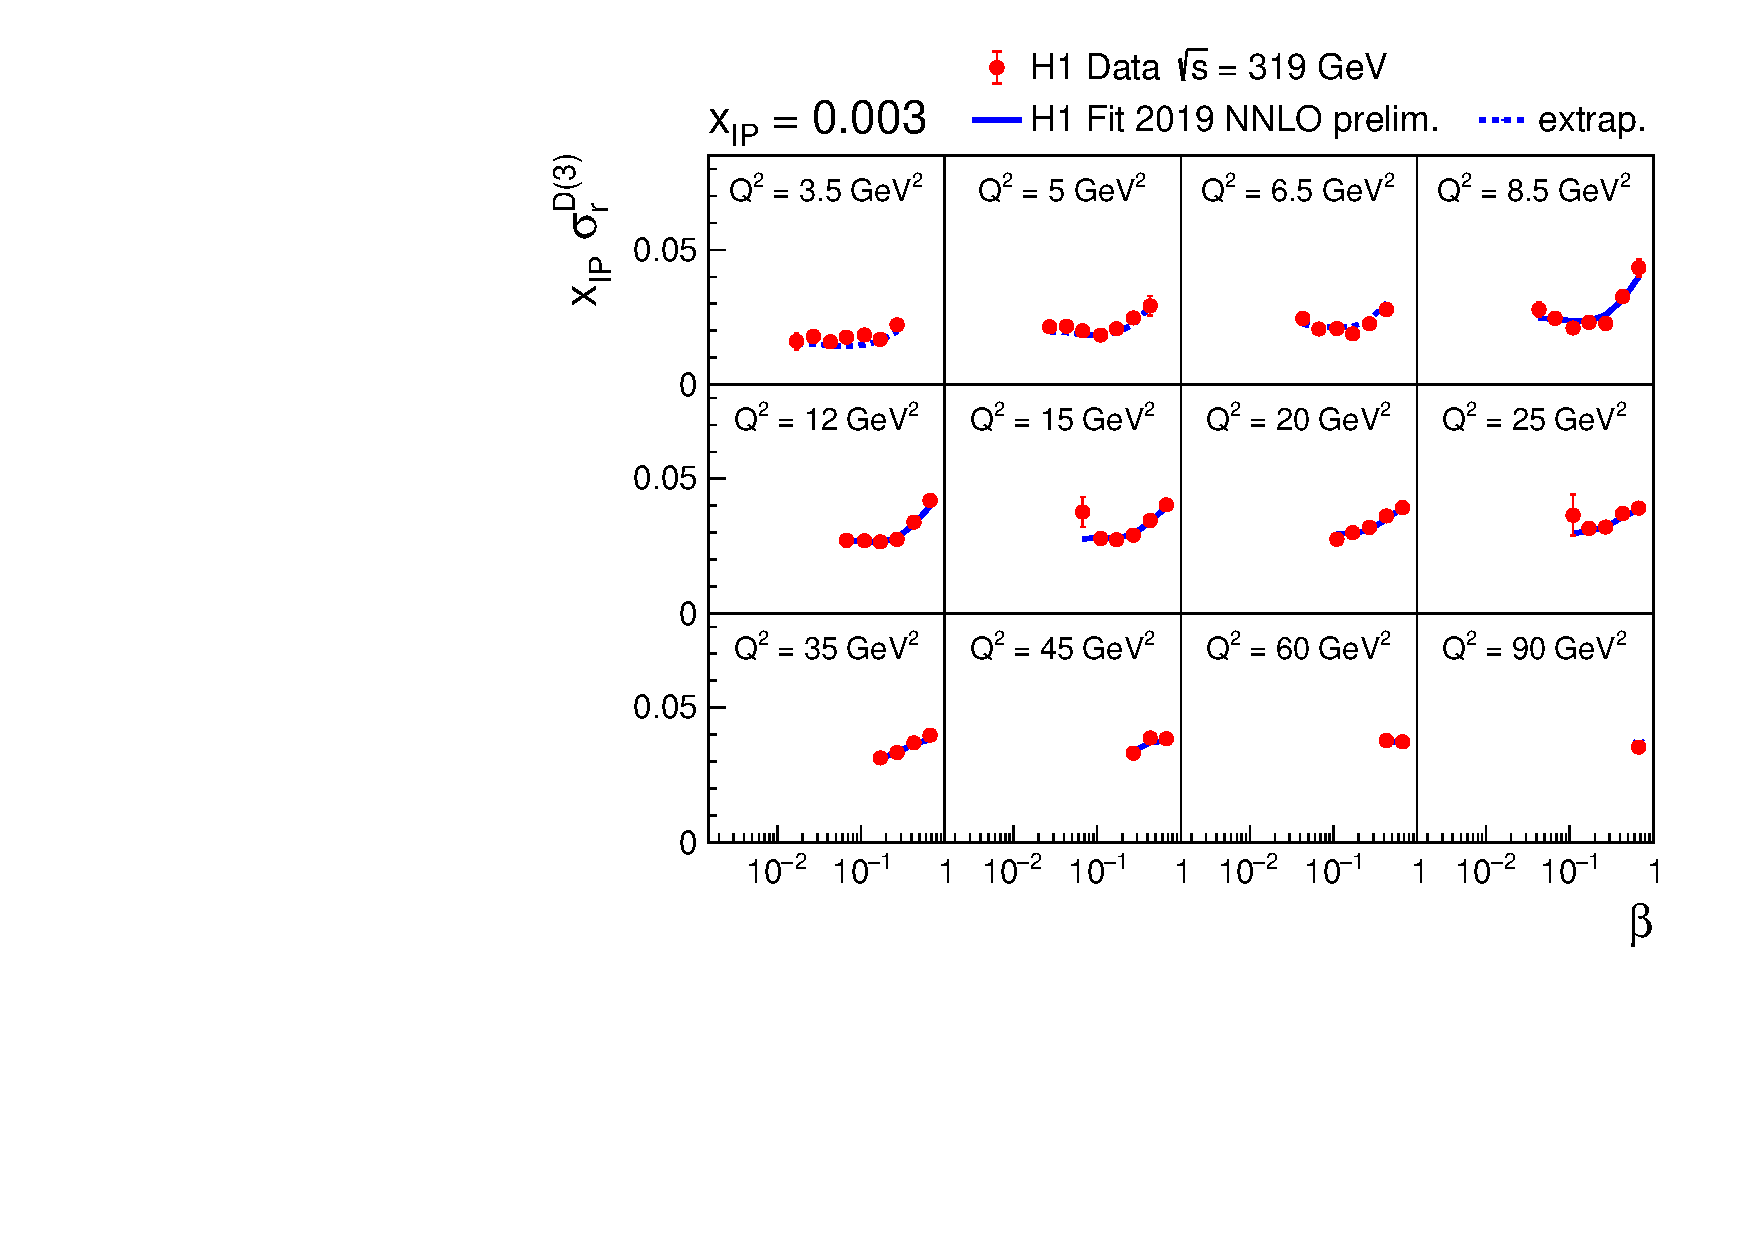
\includegraphics[width=0.8\textwidth]{{{plots/comb_beta_xpom0.003}.pdf}}
\end{center}
\caption{
  Comparison of (fitted) NNLO predictions using \DPDF\ (full line) to H1 combined LRG data as a function of $\beta$ at
  $\xpom=0.003$ (full circles).
  Other details as in fig.~\ref{fig:comb_q2_xpom0p03}.
}
\label{fig:}
\end{figure}

\begin{figure}[tbhp]
\begin{center}
  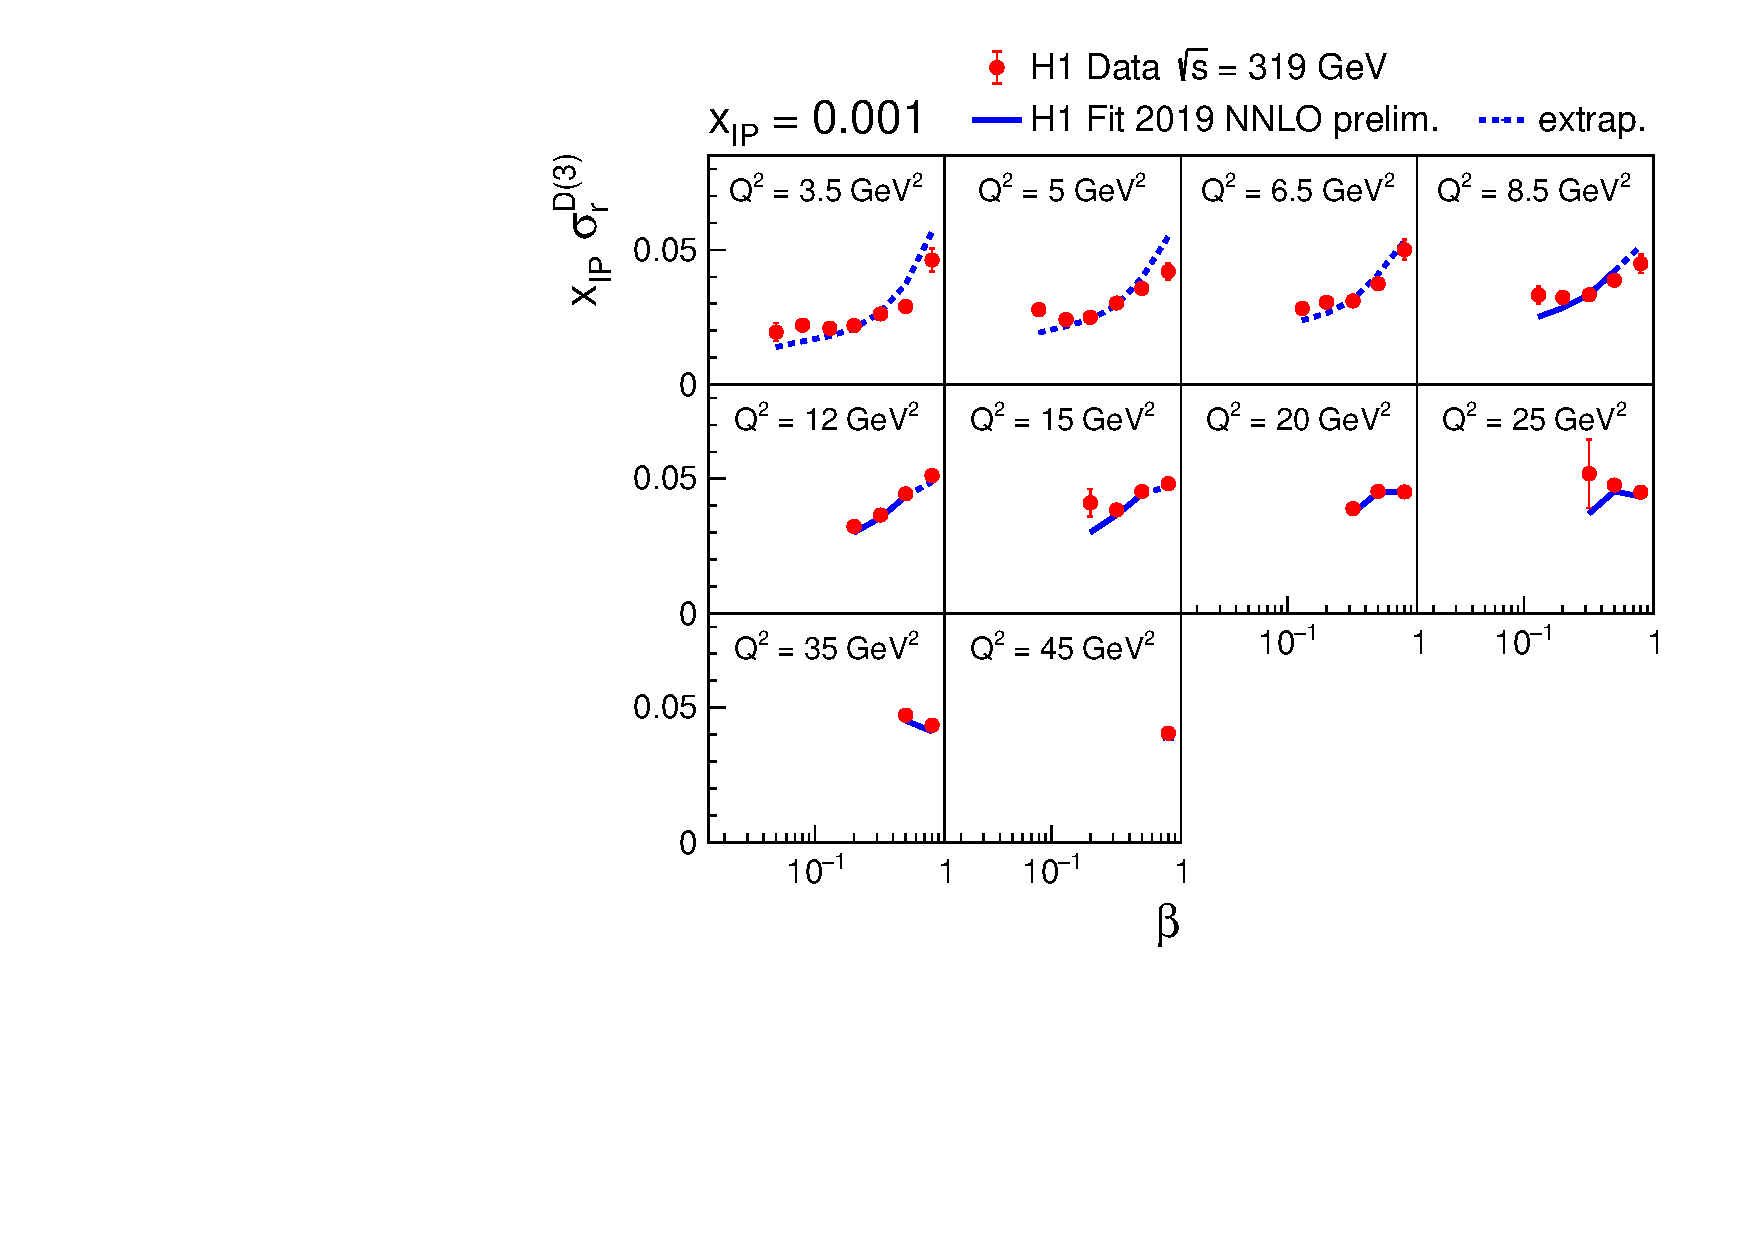
\includegraphics[width=0.8\textwidth]{{{plots/comb_beta_xpom0.001}.pdf}}
\end{center}
\caption{
  Comparison of (fitted) NNLO predictions using \DPDF\ (full line) to H1 combined LRG data as a function of $\beta$ at
  $\xpom=0.001$ (full circles).
  Other details as in fig.~\ref{fig:comb_q2_xpom0p03}.
}
\label{fig:}
\end{figure}

\begin{figure}[tbhp]
\begin{center}
  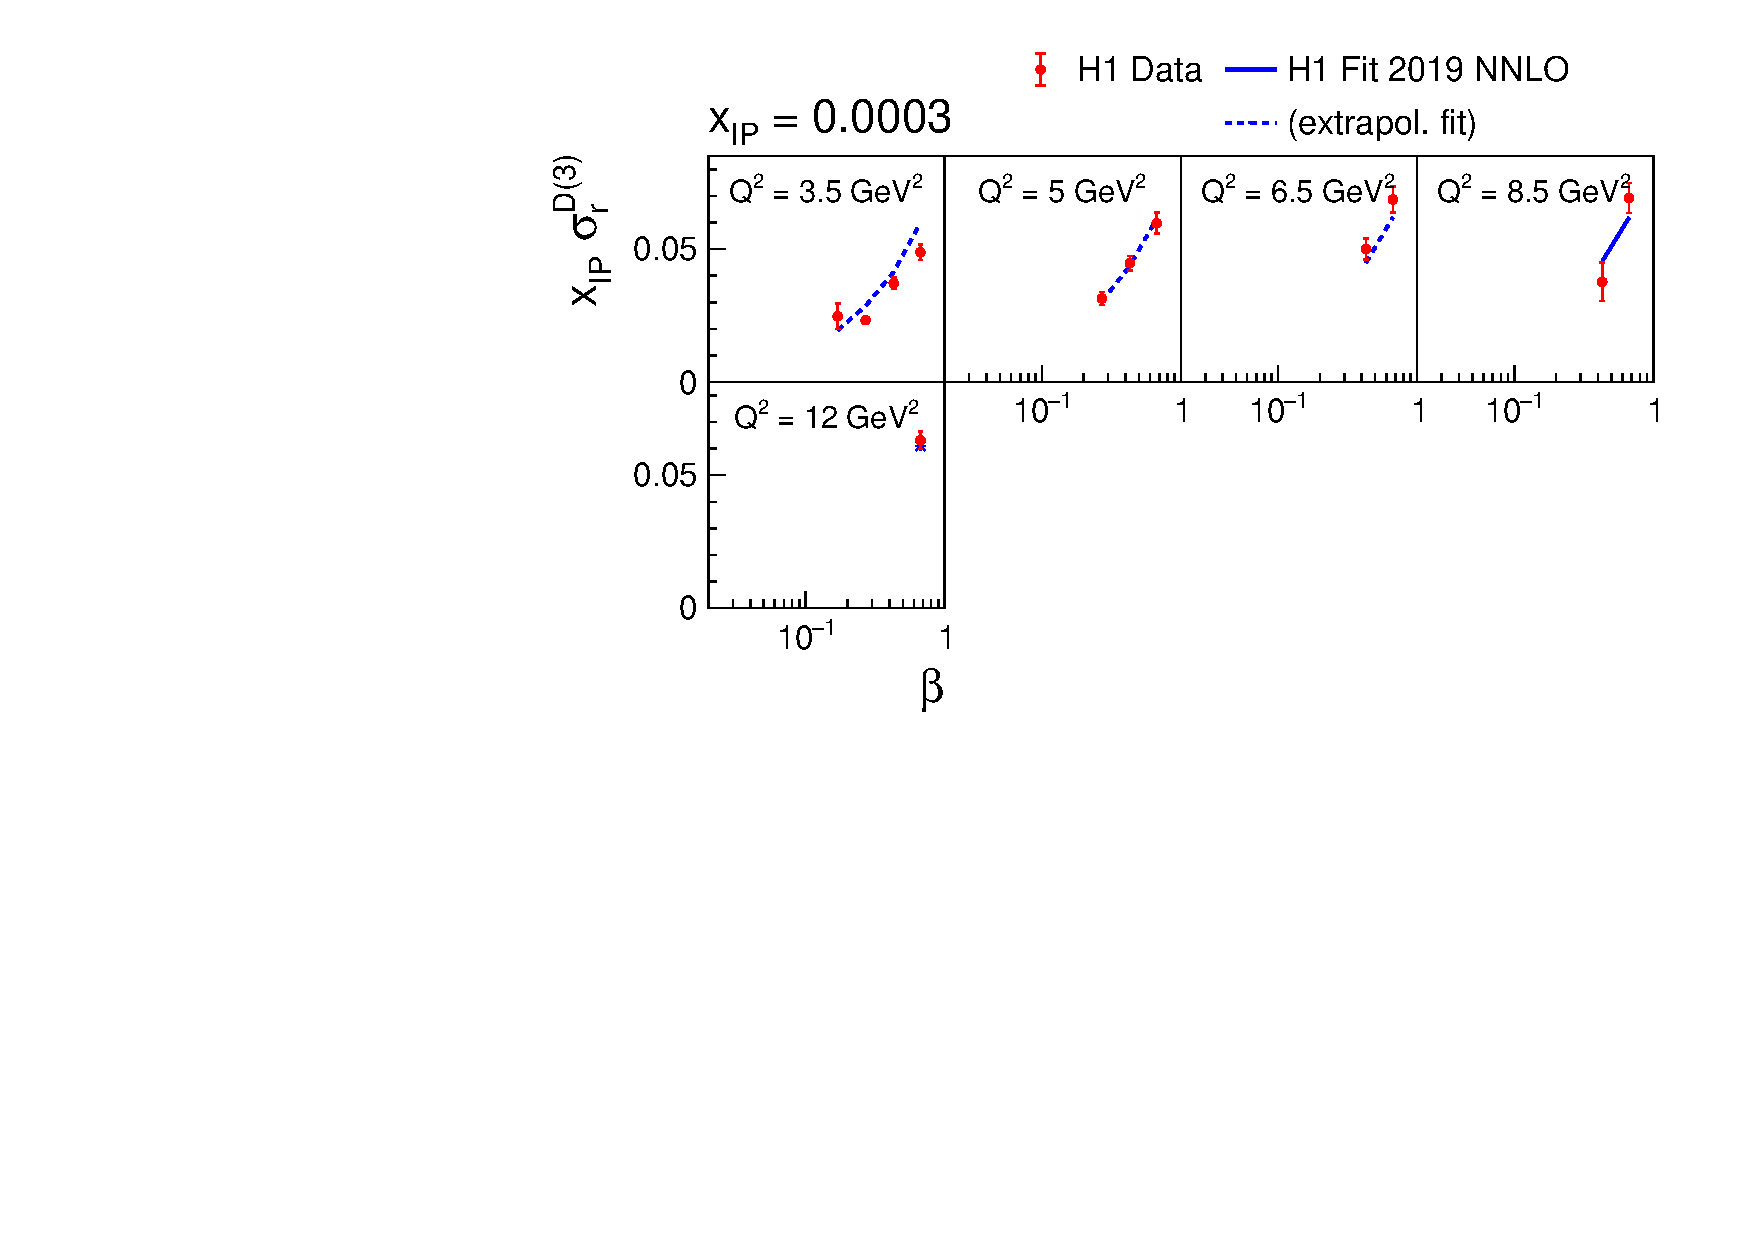
\includegraphics[width=0.8\textwidth]{{{plots/comb_beta_xpom0.0003}.pdf}}
\end{center}
\caption{
  Comparison of (fitted) NNLO predictions using \DPDF\ (full line) to H1 combined LRG data as a function of $\beta$ at
  $\xpom=0.0003$ (full circles).
  Other details as in fig.~\ref{fig:comb_q2_xpom0p03}.
}
\label{fig:}
\end{figure}



\begin{figure}[tbhp]
\begin{center}
  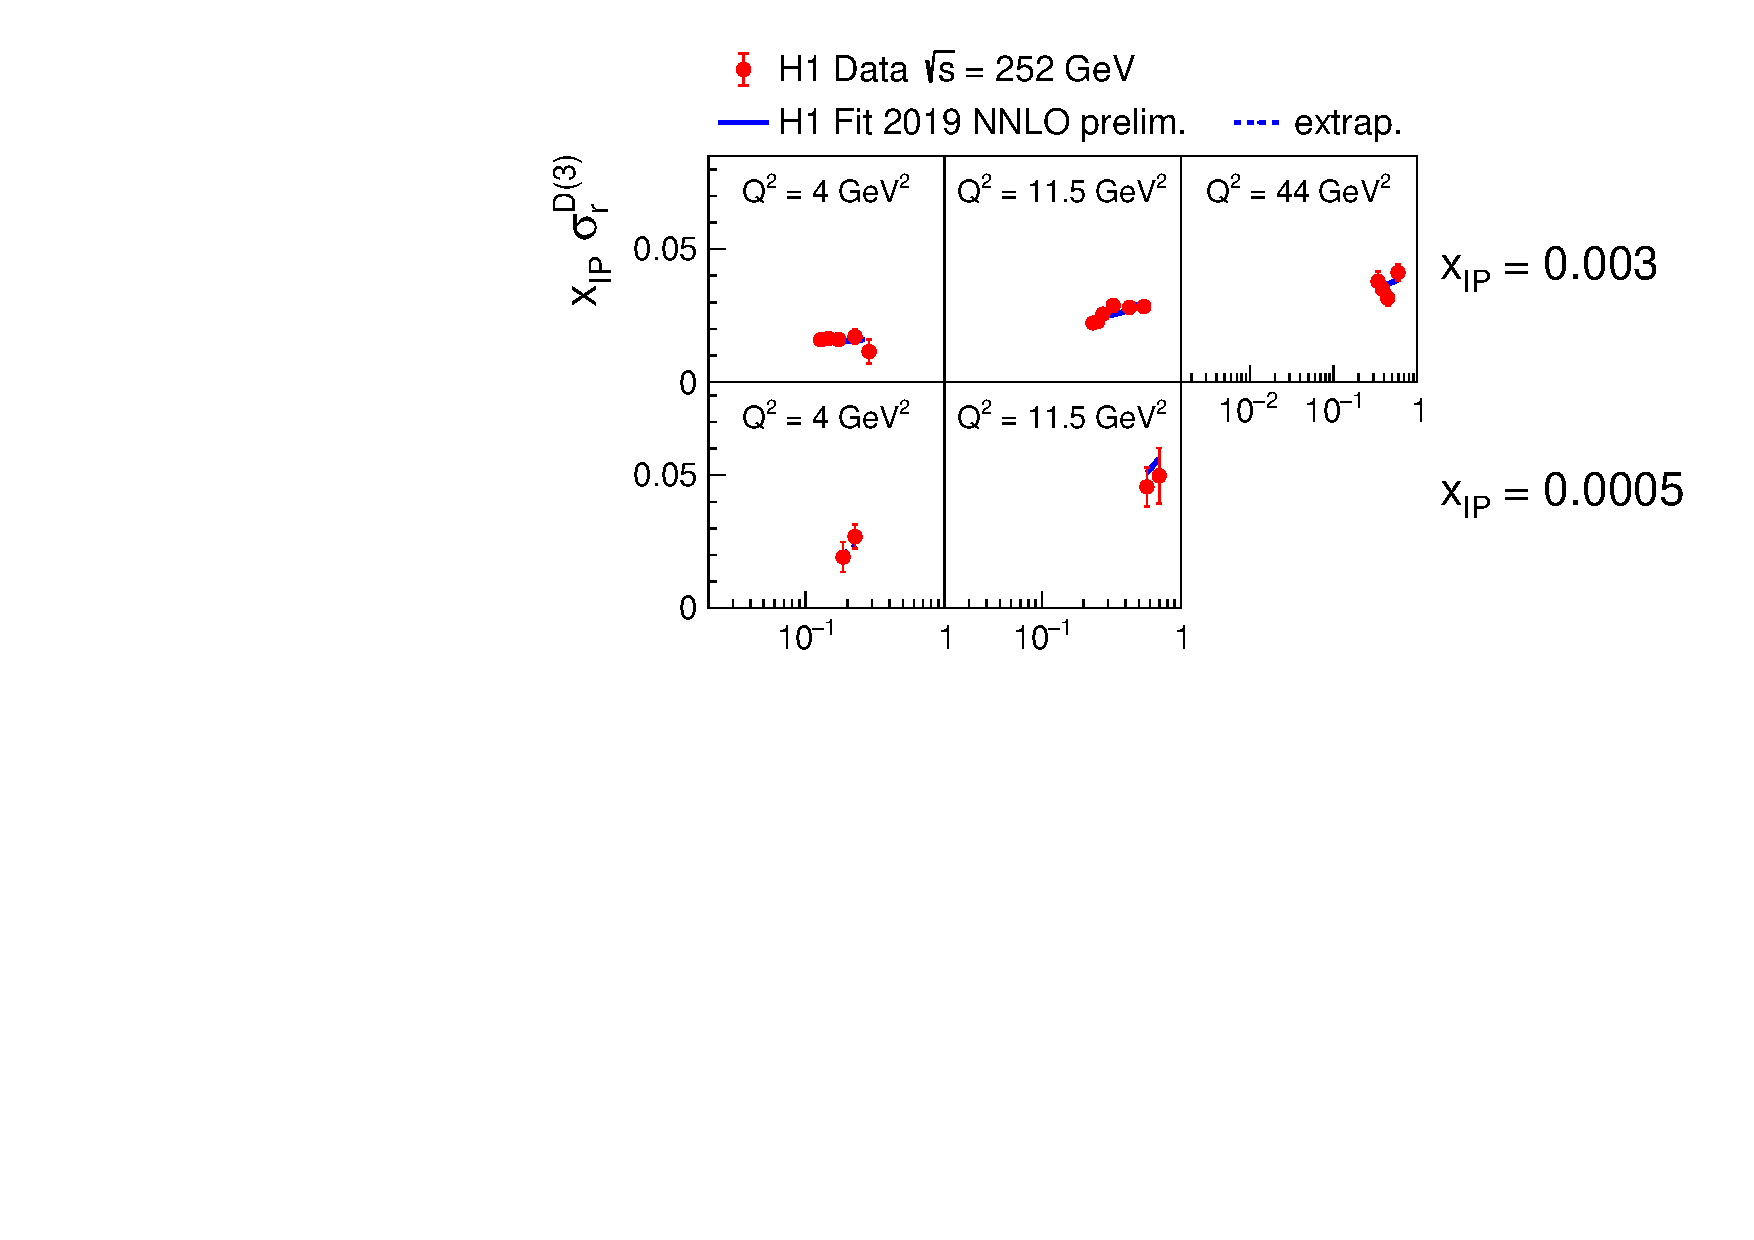
\includegraphics[width=0.8\textwidth]{{{plots/e252_betaMore_xpom}.pdf}}
\end{center}
\caption{
  Comparison of (fitted) NNLO predictions using \DPDF\ (full line) to H1 LRG data taken with $\sqrt{s}=252\,\GeV$ at  $\xpom=0.003$ and $\xpom=0.0005$ (full circles) as a function of $\beta$.
  Other details as in fig.~\ref{fig:comb_q2_xpom0p03}.
}
\label{fig:}
\end{figure}


\begin{figure}[tbhp]
\begin{center}
  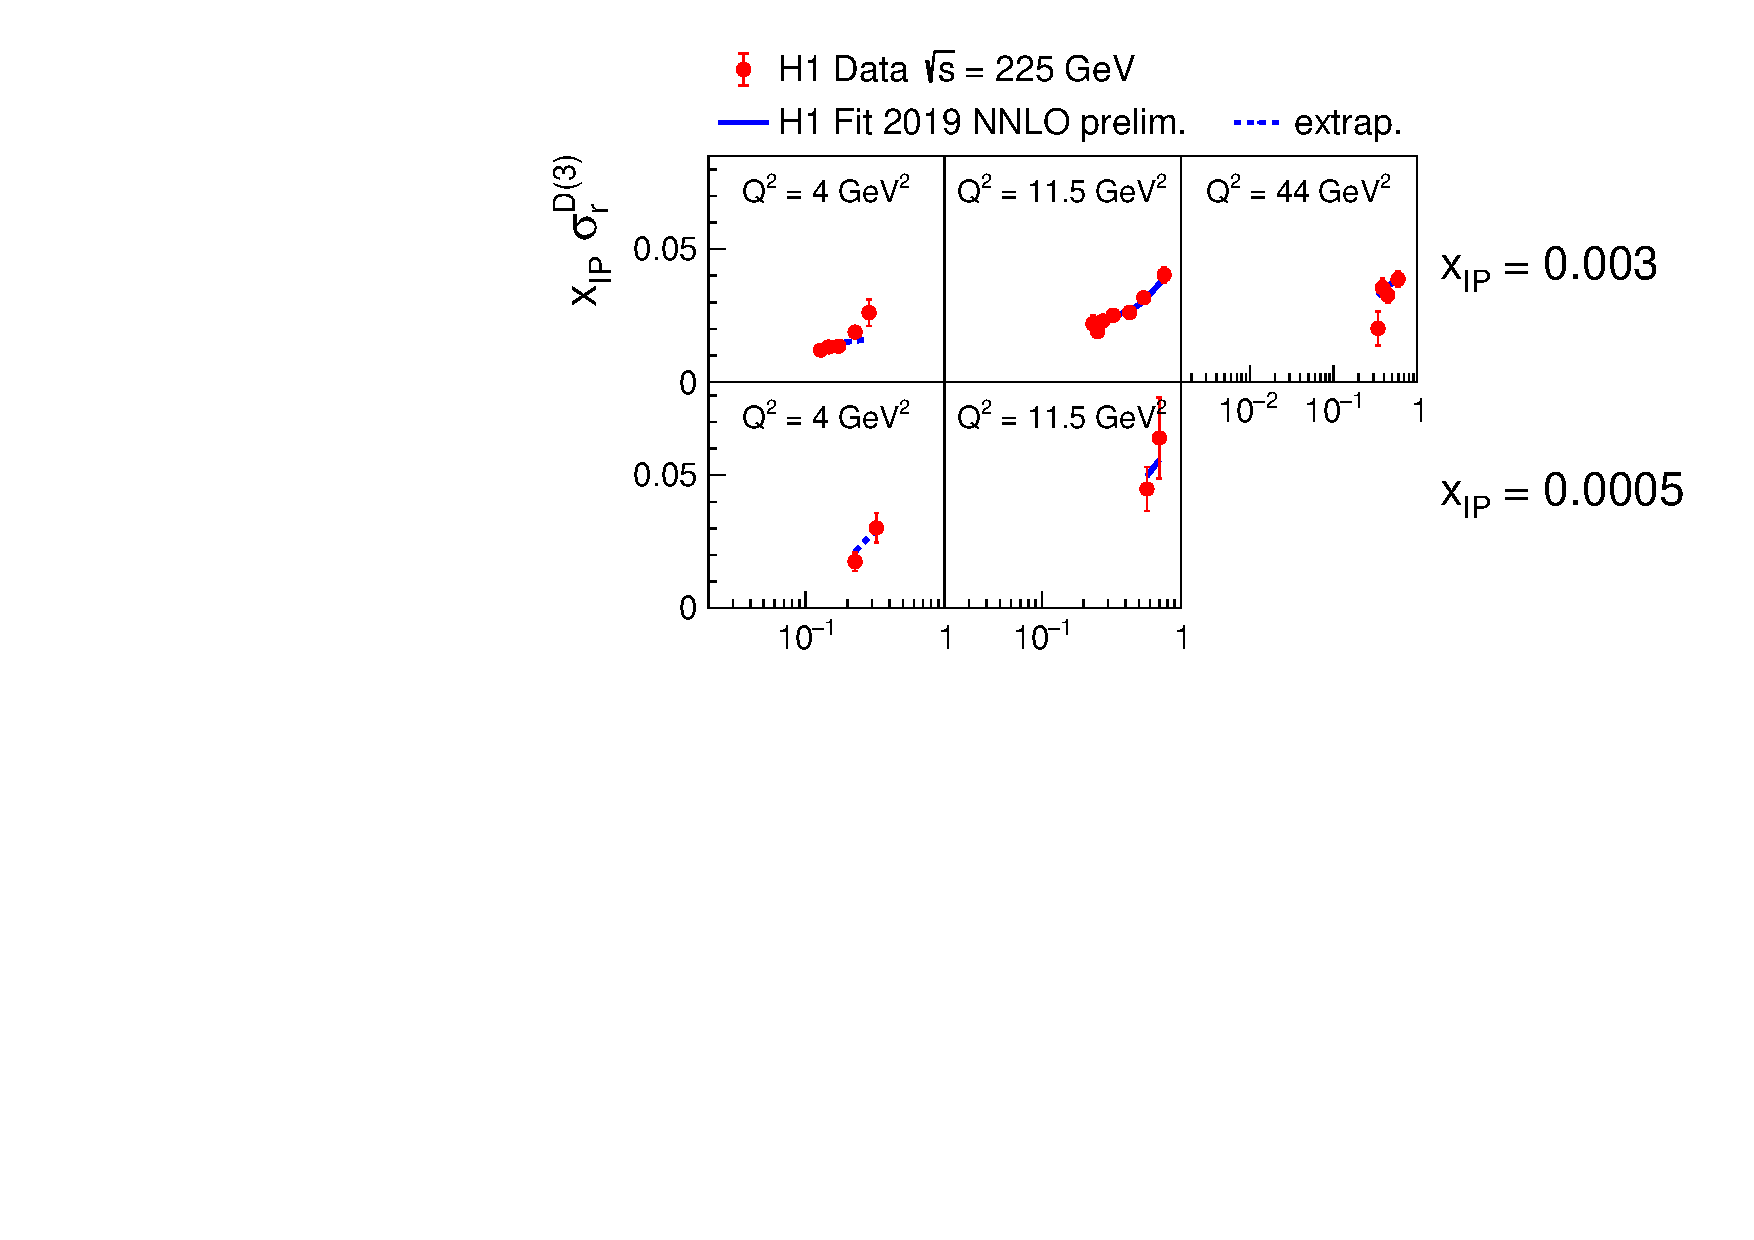
\includegraphics[width=0.8\textwidth]{{{plots/e225_betaMore_xpom}.pdf}}
\end{center}
\caption{
  Comparison of (fitted) NNLO predictions using \DPDF\ (full line) to H1 LRG data taken with $\sqrt{s}=225\,\GeV$ at  $\xpom=0.003$ and $\xpom=0.0005$ (full circles) as a function of $\beta$.
  Other details as in fig.~\ref{fig:comb_q2_xpom0p03}.
}
\label{fig:}
\end{figure}



%%%%%%%%%%%%%%%%%%%%%%%%%%%%%%%%%%%%%%%%%%%%%%%%%%%%%%%%%%%%
%                    bib
%%%%%%%%%%%%%%%%%%%%%%%%%%%%%%%%%%%%%%%%%%%%%%%%%%%%%%%%%%%%
\clearpage
\bibliography{H1prelim-19-013}




%%%%%%%%%%%%%%%%%%%%%%%%%%%%%%%%%%%%%%%%%%%%%%%%%%%%%%%%%%%%
%                    tables
%%%%%%%%%%%%%%%%%%%%%%%%%%%%%%%%%%%%%%%%%%%%%%%%%%%%%%%%%%%%
\clearpage
%\section*{Table of results}



%%%%%%%%%%%%%%%%%%%%%%%%%%%%%%%%%%%%%%%%%%%%%%%%%%%%%%%%%%%%
%                    figures
%%%%%%%%%%%%%%%%%%%%%%%%%%%%%%%%%%%%%%%%%%%%%%%%%%%%%%%%%%%%
\clearpage
%\section*{Figures}

\end{document}
